\documentclass[conference]{IEEEtran}

% ============================================================
% PACKAGES
% ============================================================
\usepackage{cite}
\usepackage{amsmath,amssymb,amsfonts}
\usepackage{algorithmic}
\usepackage{graphicx}
\usepackage{textcomp}
\usepackage{xcolor}
\usepackage{booktabs}
\usepackage{multirow}
\usepackage{hyperref}
\usepackage{tabularx}

\def\BibTeX{{\rm B\kern-.05em{\sc i\kern-.025em b}\kern-.08em
    T\kern-.1667em\lower.7ex\hbox{E}\kern-.125emX}}

\begin{document}

% ============================================================
% TITLE & AUTHORS
% ============================================================
\title{Noise-Aware Fine-Tuning of BirdNET for Indian Bird Species Classification Using the IBC53 Dataset}

\author{
\IEEEauthorblockN{Aditya S.}
\IEEEauthorblockA{
% \textit{Department of Computer Science} \\
% \textit{University Name} \\
% City, Country \\
% email@example.com
}
}

\maketitle

% ============================================================
% ABSTRACT
% ============================================================
\begin{abstract}
Automated classification of bird species through recorded sounds is an essential task in biodiversity monitoring; however, pre-trained models such as BirdNET suffer from degraded performance when applied to unrepresented regional birds' vocalisations. In this work, we introduce a novel noise-aware fine-tuning method aimed at adapting BirdNET to classify 30 Indian bird species based on the IBC53 dataset. Our methodology involves a seven-stage classification-segmentation-training (CST) pipeline consisting of segmentation of raw field recordings into 3 seconds long clips followed by their classification into the classes of bird calls, noise, or silence based on spectral characteristics (RMS energy, spectral flatness, zero-crossing rate) and data augmentation by adding examples of environmental noise from ESC-50 dataset. Experiments are carried out in four conditions: (1) a pre-trained BirdNET model, (2) fine-tuned BirdNET model, (3) fine-tuned BirdNET model with the noise class included and (4) few-shot learning using 10, 25, or 50 examples per each species. Results indicate that noise-aware training leads to improved performance from 74.56\% to 75.61\%, accompanied by increase in median prediction confidence by 71\% (from 0.43 to 0.74), reducing a number of false positives by 510. Analysis of few-shot experiments indicates a performance of 60.86\% with 50 samples per species, which suggests reasonable effectiveness of the approach in the context of limited data. Finally, we identify persistent species-specific confusion between morphologically similar babblers as resulting from the spectral similarity.
\end{abstract}

\begin{IEEEkeywords}
bioacoustics, bird species classification, BirdNET, transfer learning, noise-aware training, few-shot learning, Indian avifauna, ESC-50
\end{IEEEkeywords}

% ============================================================
% I. INTRODUCTION
% ============================================================
\section{Introduction}

India is home to more than 1,350 bird species in different ecological regions, including Himalayan alpine tundra and tropical coastal mangrove forests \cite{b7}. However, many of these species exhibit acoustic distinctiveness but pose problems regarding taxonomy. For instance, the family Timaliidae comprises several species that share similar frequency responses despite being sympatric. IBC53 is a bird sound dataset collected from the Internet Bird Collection database containing recordings of 53 bird species from India. IBC53 allows the researchers to experimentally assess the performance of pre-trained models on an under-studied dataset. Initial experiments using BirdNET on IBC53 data reveal two critical failure cases, which include: (i)~The pre-trained models make confident predictions for bird species not included or sparsely included in the training set; and (ii)~Noise segments (including rainfall, wind, and insect chirping) are incorrectly predicted as bird calls.

Fine-tuning-based transfer learning offers a formalized methodology for domain adaptation \cite{b8}. Fine-tuning of the classifier head using target-domain data while preserving the pre-trained feature extractor ensures quick adaptation of the general purpose model to a novel species community using a small labeled dataset. On the other hand, a naive fine-tuning scheme based only on bird recordings fails to tackle the issue of noise. With no negative samples available, the output softmax layer will have to classify every sample as one of the birds. It becomes an even bigger challenge for field recordings, where each sample is likely to have significant sections that contain silence, wind, rain, or man-made noise. This paper proposes a fine-tuning technique that takes into account environmental noise during training. We introduce a seven-step C-STT pipeline, which includes: (1)~segmentation of the raw field recordings in 3-second blocks matching the input size expected by BirdNET; (2)~classification of every block as bird vocalization, noise, or silence using the RMS energy, spectral flatness, and zero-crossing rate (ZCR); (3)~augmentation of the training data with labeled environmental noises from the ESC-50 dataset \cite{b2}; and (4)~fine-tuning of BirdNET's classifier on the expanded 31-class dataset (30 species + noise).

We evaluate four experimental conditions to isolate the contributions of fine-tuning and noise-aware training:

\begin{itemize}
    \item \textbf{Baseline}: Pre-trained BirdNET without any further fine-tuning, testing its out-of-distribution generalisation capabilities with respect to Indian species.
    \item \textbf{Experiment~1}: Fine-tuning on 30 species \textit{without} a noise class to estimate the impact of domain adaptation only.
    \item \textbf{Experiment~2}: Fine-tuning on 30 species \textit{with} an explicit noise class to estimate the additional value of noise-aware training.
    \item \textbf{Experiment~3}: Few-shot fine-tuning with 10, 25, and 50 samples per class with noise to explore the minimum amount of data required for training and data efficiency.
\end{itemize}

The major contributions of this study are:

\begin{enumerate}
    \item A reproducible, modular CST process for field recordings preparation for BirdNET fine-tuning, featuring automated detection of noise/silence and usage of ESC-50.
    \item Empirical proof of better classification performance (+1.05 percentage points) and, most importantly, significant increase of median prediction confidence by 71\% and, thus, decrease of false detections by 510.
    \item Analysis of few-shot setting showing that 50 labeled samples per species provide 60.86\% accuracy and, therefore, establishing a minimal dataset size threshold.
    \item Identification and analysis of confusion between different species of Indian babblers (Timaliidae) caused by their spectral similarities rather than noise, thus identifying the limit between data engineering and model architecture.
\end{enumerate}

The remainder of this paper is organised as follows. Section~II reviews related work in bioacoustic classification and transfer learning. Section~III details the proposed methodology and pipeline design. Section~IV describes the experimental setup. Section~V presents results and comparative analysis. Section~VI discusses findings, limitations, and future directions. Section~VII concludes the paper.

% ============================================================
% II. RELATED WORK
% ============================================================
\section{Related Work}

BirdNET was evaluated for its accuracy compared to experts by means of recordings from Munich, Germany with different parameter settings, which affected its performance with a wide range from 0.46 to 0.84 in terms of precision, recall and F1 scores; and with higher temporal aggregation, optimal tuning of sensitivity, week of year and 1--2 seconds overlap, BirdNET almost equaled experts' results at F1 score~=~0.84, with confidence threshold affecting the results the most, demonstrating the effectiveness of basic validation to make BirdNET feasible without specific species' confidence levels given by Fairbairn, et al~\cite{b9} (2025). The need for Species-Specific Confidence Thresholds is due to manual annotation being required, and the sample pool used for labeling affects predictions. Hence, using 33 bird species in Europe, the authors present their approach to determine the number of labeled samples required to predict consistently ecological parameters and reduce bias in the community level predictions downstream given by Petry, et al~\cite{b10} (2026). The experiment involved a comparison of point counts, manually analyzed PAM surveys, and BirdNET for Bia\l{}owie\.{z}a primaeval forest in Poland, whereby BirdNET, using full day recordings, identified the most alpha richness with 80 species, compared to 49 species through 10-minute point counts and 61 species by manually analyzing recordings, whereas beta diversity was dependent on location and approach, and the correlation between short surveys and all-day BirdNET alpha richness was low, revealing that long-term automated monitoring offers better cumulative biodiversity, yet manual analysis is crucial by Winiarska, et al~\cite{b11} (2025). World-wide BirdNET assessment based on 4,224 one-minute recordings collected at 67 locations on all continents and annotated by regional specialists, wherein precision was high and comparable on both continents at 0.57--0.71 and biomes at 0.55--0.76, but recall was relatively low and variable on continents at 0.24--0.52, with predictive capacity being optimal on North America, Oceania, and Europe but poor on Africa and Asia, and confidence thresholds being highly varied depending on species and objectives by P\'{e}rez-Granados, et al~\cite{b12} (2025). Two-year audio recordings in western Canada were used for the evaluation of two thresholding methods, whereby the common threshold of 0.7 had a precision of 0.7--1.0 but managed only 17~$\pm$~14\% of detections compared to the species-specific threshold for $\geq$0.9 precision, which resulted in 70~$\pm$~37\% of detections; the species-specific thresholds were generally $<$0.35 and unrelated to song complexity given by Tseng, et al~\cite{b13} (2025). Used the PAM and BirdNET models to analyze the wetland habitat developed on an abandoned limestone quarry in central Spain for three consecutive years, investigating the impact of Overlap and Sensitivity on the outcome of a bird inventory study; high Sensitivity generated the optimum solution through minimizing the number of species lost in the inventory, and Recall was determined as the best criterion given by Iglesias-Merchan, et al~\cite{b14} (2026). Illustrates how embeddings generated from BirdNET can identify novel sound classes not present in the training data of the model while requiring very few calls and little validation, demonstrating this by presenting three case studies -- identifying a non-native reptile species (Asian house gecko) in Christmas Island, compiling lists of amphibians and mammals using Australian Acoustic Observatory datasets, and recognizing a critically endangered bird species (Blue-winged parrot), where the method was effective across various taxa and datasets, and allowed for fast detection without having specific recognizers given by Allen-Ankins, et al~\cite{b15} (2025).

Explains the reasons for misclassification of BirdNET, comparing it with another model based on ResNet, along with the use of XAI methods such as LIME and dimensionality reduction via t-SNE and PCA to visualize the latent space, finding major class imbalances and label noises in the training datasets, particularly for hard-to-classify classes, and conducting controlled experiments to show that decreasing label noise increases the F1 score given by Assarzadeh, et al~\cite{b16} (2025). Assessing BirdNET for monitoring three Neotropical wetland birds, Green Ibis, Limpkin, and Sunbittern, in Brazil's Pantanal region throughout one year, BirdNET correctly identified the presence of birds in 82--92\% of the recordings, with precision ranging between 77\% and 98\%, where maximum vocal activity occurred during crepuscular periods, while the seasonal peaks were observed at the end of the rainy season and receding season when nesting-flooding risks were minimized and resources were plentiful provided by P\'{e}rez-Granados, et al~\cite{b17} (2025). Evaluating the effectiveness of BirdNET for detecting the Chinese Bamboo Partridge, an endemic bird, and developing a Random Forest (RF) model based on BirdNET outputs, BirdNET-Analyzer recall rate was found to be only 16.6\%, while RF model recall improved this value to 75.2\% with 74.4\% precision, with diurnal vocal activities having a bimodal pattern with peaks in sunrise and sunset hours, whereas seasonal vocal activities had a unimodal distribution, with maximum activity in April--May provided by Mei, et al~\cite{b18} (2026). Study involving monitoring two co-existing species of gulls at La Mata coastal lagoon in Spain, specifically the Yellow-Legged Gull and the IUCN-listed vulnerable Audouin's Gull, through deploying an IoT-based system powered by AI for listening and automatic classification of birds based on their sound, as described in the paper that examines methodology and explains why BirdNET should be tuned to meet this objective given by Seye, et al~\cite{b19} (2025). Testing BirdNET on bird species typical to the Alpine regions of Italy through evaluating fine-tuning techniques on regional soundscape data augmented through manual annotation, where BirdNET's fine-tuned version on regional soundscape significantly beat both the original BirdNET and a simple CNN that used only the regional soundscape data for training given by Schiavo, et al~\cite{b20} (2025). Proposes a custom classifier for BirdNET to inversely classify wind noises in recordings of Ad\'{e}lie penguins from their colonies in Antarctica using several custom classifiers for Ad\'{e}lie calls in nontarget background along with low, medium, and high wind noises as target classes, where the default training configuration beats BirdNET autotune as hyperparameter optimization cannot be achieved for unpredictable wind noises, and outlines a six-step framework for custom BirdNET model development proposed by Fradet, et al~\cite{b21} (2025).

% ============================================================
% III. PROPOSED METHODOLOGY
% ============================================================
\section{Proposed Methodology}

This study proposes a noise-aware fine-tuning framework for BirdNET-based avian species classification, specifically designed to improve recognition accuracy on the Indian Bird Call dataset (IBC53) comprising 30 species. The proposed pipeline integrates domain-specific audio preprocessing with transfer learning on the BirdNET deep learning backbone. The framework consists of four principal stages: (1)~audio segmentation, (2)~energy-based noise detection, (3)~noise-augmented dataset construction, and (4)~BirdNET fine-tuning with multi-configuration evaluation. The overall architecture of the proposed methodology is depicted in Fig.~\ref{fig:architecture}.

\begin{figure}[htbp]
\centerline{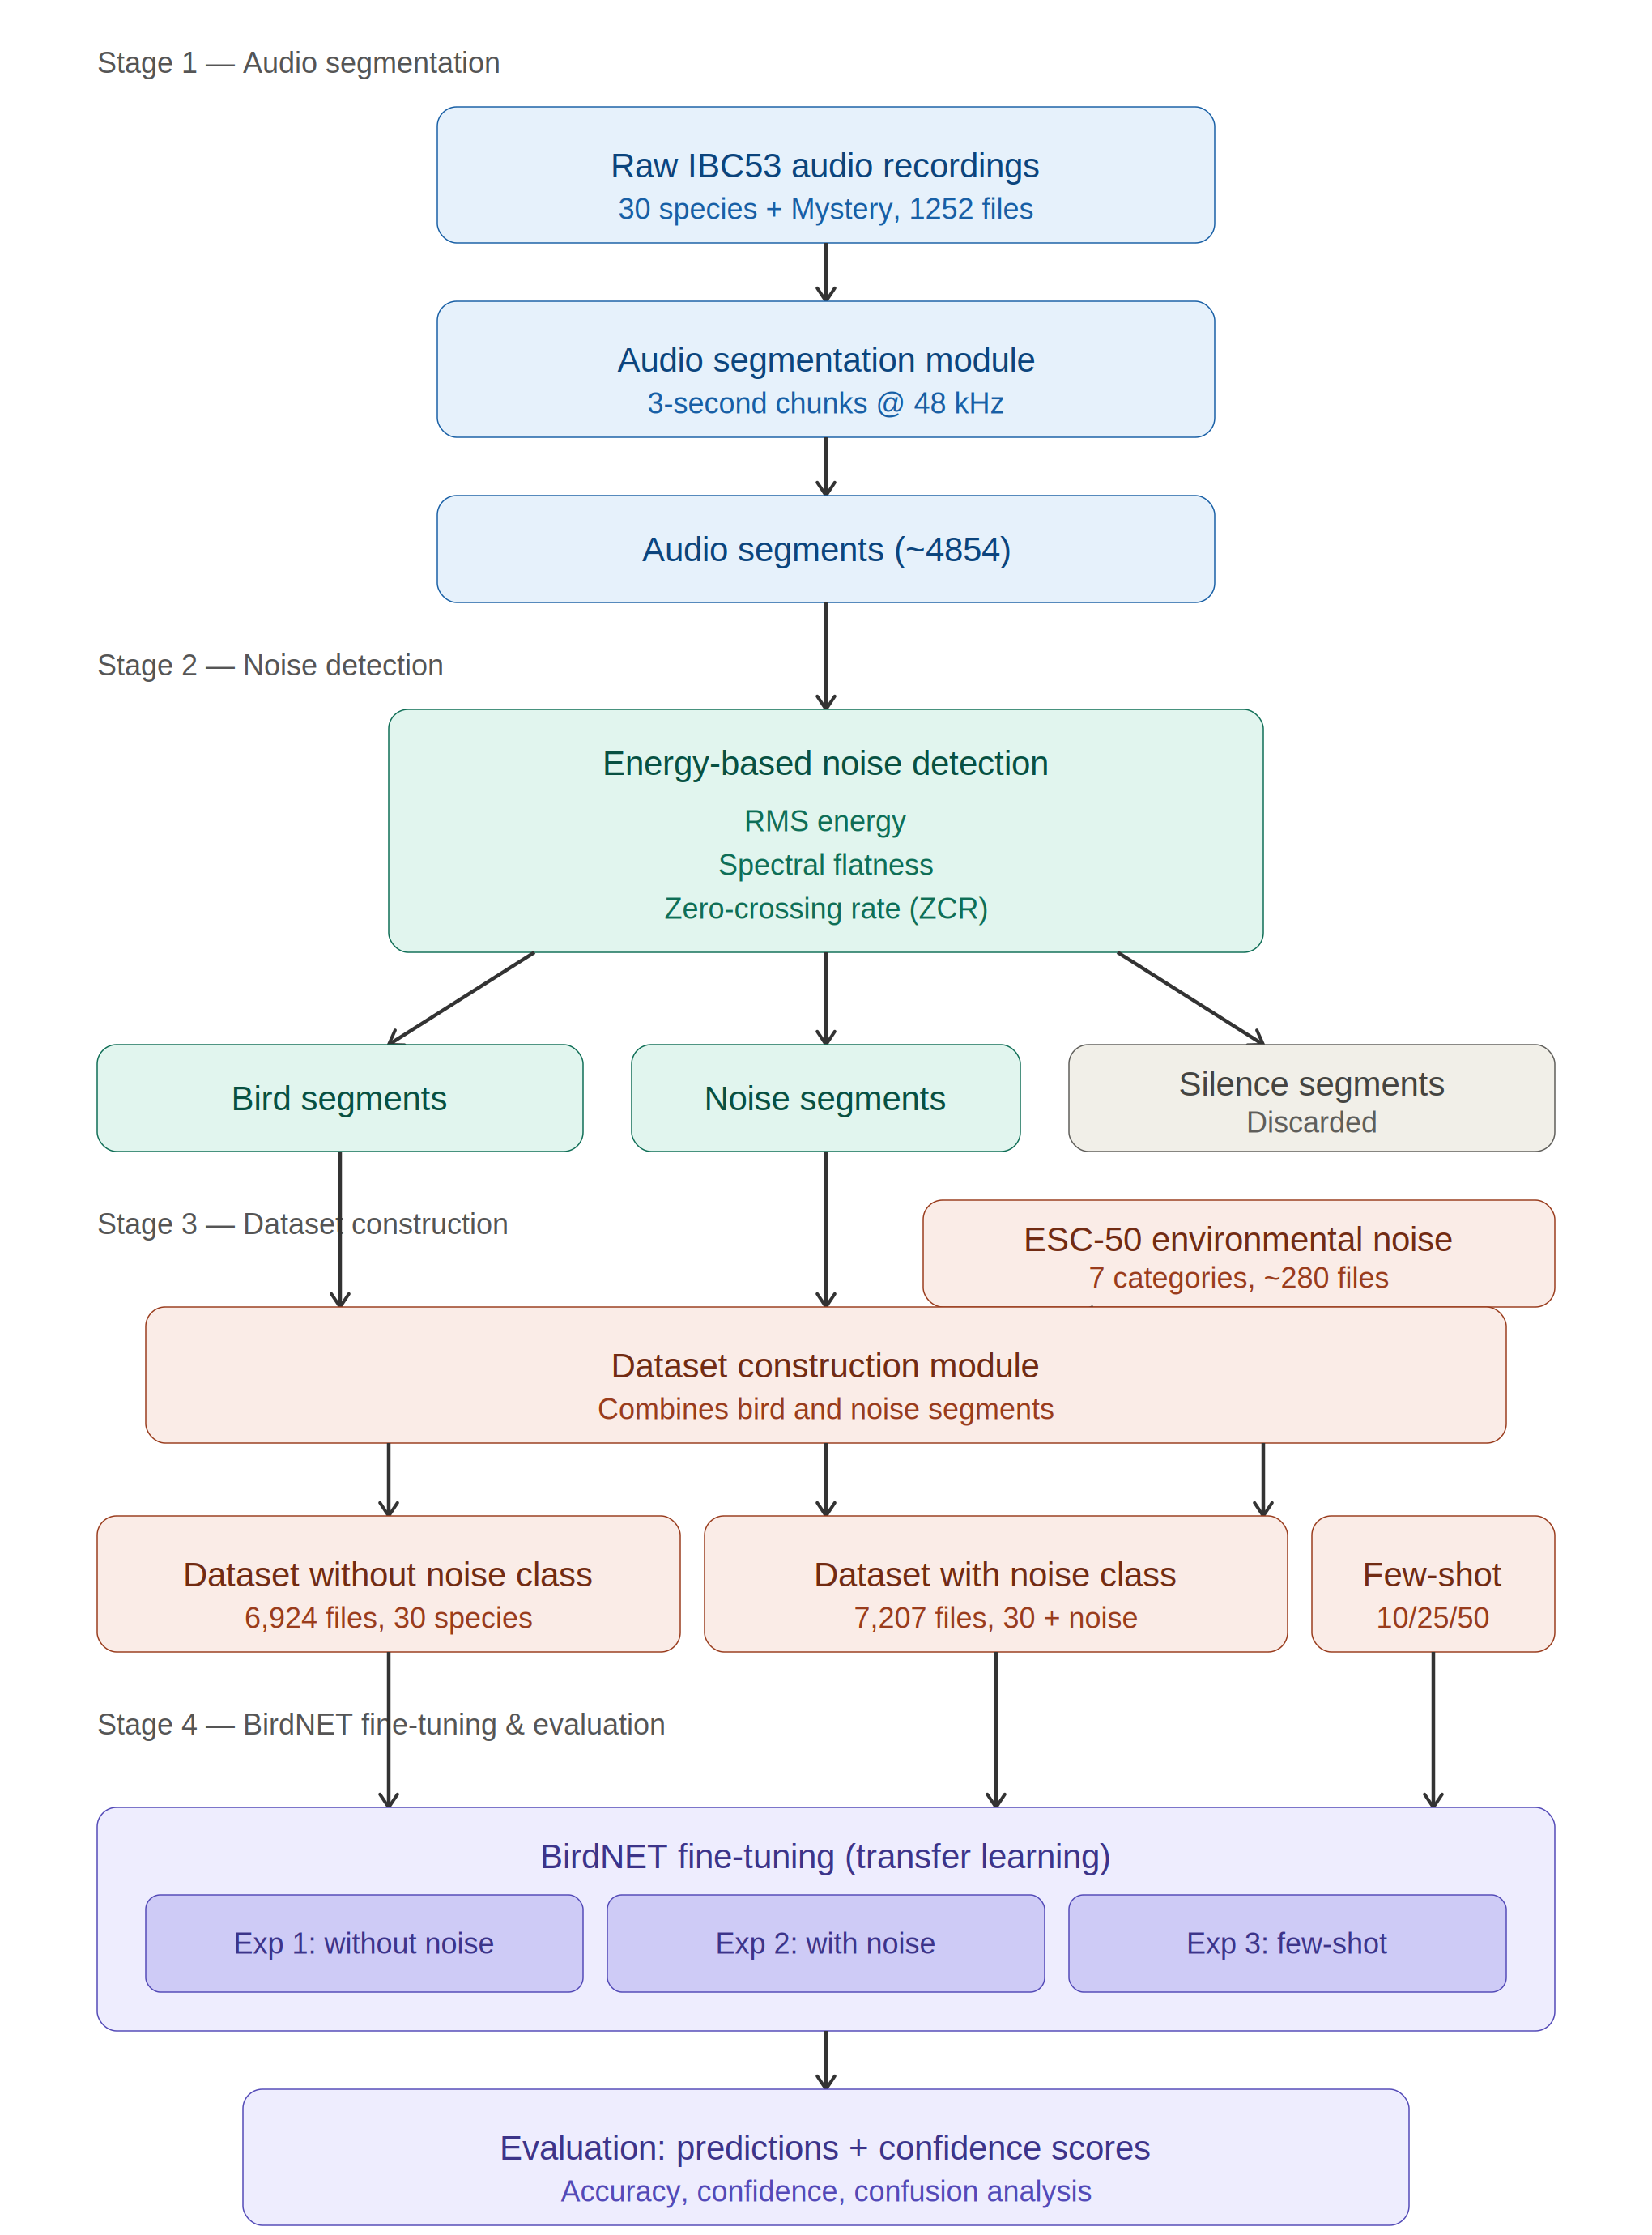
\includegraphics[width=\columnwidth]{figures/birdnet_pipeline_architecture.png}}
\caption{Architecture of the proposed noise-aware BirdNET fine-tuning framework showing the four-stage pipeline: audio segmentation, energy-based noise detection, dataset construction with ESC-50 noise integration, and BirdNET fine-tuning with multi-experiment evaluation.}
\label{fig:architecture}
\end{figure}

\subsection{Audio Segmentation}

The initial step in the proposed pipeline involves tackling the problem of handling varying lengths of field recordings in order to generate consistent input samples that can be used by the classifier based on deep learning models. The audio recordings obtained from the IBC53 dataset, consisting of a total of 1,252 recordings from 30 Indian bird species and another 443 mystery recordings without labels, are divided into samples of equal length of 3 seconds.

The process of segmentation makes use of a simple non-overlapping sliding window technique. First, the waveform in each audio recording is resampled to a rate of 48~kHz since this is the input size accepted by BirdNET. The resampled waveform is subsequently divided into sequential 3-second samples. Any waveform less than 3 seconds in length at the end of a recording is zero-padded in order to maintain dimensional consistency. With this process, the original 1,252 recordings are converted to approximately 4,854 samples. If we let $x(t)$ represent the audio recording waveform of duration $T$ seconds, the segmentation operator $S$ produces $N$ segments of length $L = 3$, where $N = \lceil T / L \rceil$, such that each segment $s_i$ can be expressed as:

\begin{equation}
s_i = x(t), \quad t \in [3(i-1),\; 3i], \quad i = 1, 2, \ldots, N
\end{equation}

In cases where the duration of the last frame is less than three seconds, zero padding is used so that the length of all the frames becomes 144,000 samples ($3 \times 48{,}000$~Hz).

\subsection{Noise Detection Based on Energy}

A field recording will have a mix of target bird vocalization, environmental noise, and silence in every recording. Training the classifier on these segments will result in label noise and reduce classifier performance. This challenge will be addressed in the second phase through the implementation of an energy-based noise detection module where each of the 3-second segments will be categorized as follows: bird vocalization, environmental noise, or silence.

Each of the 3-second segments will be classified based on three acoustic features calculated from both time domain and frequency domain:

\subsubsection{RMS Energy}
RMS Energy calculates the average energy in the audio signal. A segment is said to be silence if its RMS energy level is below the threshold value of $\theta_{\mathrm{RMS}} = 0.01$ since it does not have enough energy content. The RMS energy calculation formula for a sample $s_i$ of length $L$ is given by:

\begin{equation}
\mathrm{RMS}(s_i) = \sqrt{\frac{1}{L} \sum_{n=0}^{L-1} s_i[n]^2}
\end{equation}

\subsubsection{Spectral Flatness}
The spectral flatness feature characterizes how evenly distributed the power spectrum is. A high spectral flatness corresponds to a uniformly distributed power spectrum, resembling the spectrum of a noise-like signal (white noise). Conversely, low spectral flatness values correspond to spectra that have distinct peaks, which is a feature typical for tonal signals like bird calls. The spectral flatness can be calculated as the ratio of the geometric mean of the power spectral density to its arithmetic mean. The noise segments are identified using segments that have spectral flatness above the threshold $\theta_{\mathrm{SF}} = 0.5$.

\begin{equation}
\mathrm{SF}(s_i) = \frac{\left(\prod_{k=0}^{K-1} P(k)\right)^{1/K}}{\frac{1}{K} \sum_{k=0}^{K-1} P(k)}
\end{equation}

\noindent where $P(k)$ is the power spectral density of the $k$th frequency bin, and $K$ is the total number of frequency bins.

\subsubsection{Zero-Crossing Rate (ZCR)}
This measure refers to the rate at which the signal crosses the zero axis in its amplitude domain. As noise signals are aperiodic and unpredictable, their ZCR values are generally higher than those of bird songs. Segments that have spectral flatness greater than $\theta_{\mathrm{SF}}$ and ZCR greater than $\theta_{\mathrm{ZCR}} = 0.1$ are considered noise.

\begin{equation}
\mathrm{ZCR}(s_i) = \frac{1}{2L} \sum_{n=1}^{L-1} \left| \mathrm{sign}(s_i[n]) - \mathrm{sign}(s_i[n-1]) \right|
\end{equation}

The combined decision rule for segment classification is formulated as follows: a segment is labeled as silence if $\mathrm{RMS}(s_i) < \theta_{\mathrm{RMS}}$; as noise if $\mathrm{SF}(s_i) > \theta_{\mathrm{SF}}$ AND $\mathrm{ZCR}(s_i) > \theta_{\mathrm{ZCR}}$; and as bird vocalization otherwise. Table~\ref{tab:thresholds} summarizes the threshold parameters used in the noise detection module.

\begin{table}[htbp]
\caption{Threshold Parameters for Energy-Based Noise Detection}
\label{tab:thresholds}
\centering
\begin{tabular}{lccc}
\toprule
\textbf{Parameter} & \textbf{Symbol} & \textbf{Value} & \textbf{Purpose} \\
\midrule
RMS Threshold & $\theta_{\mathrm{RMS}}$ & 0.01 & Silence detection \\
Spectral Flatness Threshold & $\theta_{\mathrm{SF}}$ & 0.5 & Noise candidate detection \\
Zero-Crossing Rate Threshold & $\theta_{\mathrm{ZCR}}$ & 0.1 & Noise confirmation \\
\bottomrule
\end{tabular}
\end{table}

\subsection{Training Data Set Creation with Noise Augmentation}

The final stage involves the generation of training data sets that will be used in fine-tuning BirdNET. This is an important addition to the paper, whereby special care has been taken to include noise samples in the training data set to allow the model to learn noise suppression when making predictions.

The bird call samples filtered in Stage~2 are sorted into separate directories for each type of bird according to the expected training data set format for BirdNET, where the subdirectories are named by the scientific name of the bird (e.g., \textit{Pnoepyga\_pusilla}, \textit{Pellorneum\_ruficeps}). This gives a data set of 6,924 samples for 30 bird species classes.

To create the noise-augmented dataset, environmental noise samples are taken from the ESC-50 \cite{b2} dataset. Noise classes that are applicable to field recording scenarios are chosen, specifically: rain, wind, thunderstorm, insects, water drops, crackling fire, and engine idling. In total, 283 noise samples are obtained and stored in a special noise folder. During training, BirdNET sees this folder as a \texttt{NON\_EVENT\_CLASS} which means that the noise samples do not have a dedicated output label but rather help to train BirdNET to ignore non-bird sound snippets. The noise-augmented dataset includes 7,207 audio files (6,924 birds + 283 noises).

Besides, few-shot samples are taken from the whole dataset in order to evaluate data efficiency. In particular, for each of 30 species and noise class, samples of 10, 25, and 50 samples are taken randomly and without replacement leading to the creation of 3 few-shot datasets including 583, 1,033, and 1,783 samples respectively. Table~\ref{tab:datasets} summarizes the dataset configurations.

\begin{table}[htbp]
\caption{Dataset Configurations for Experimental Evaluation}
\label{tab:datasets}
\centering
\begin{tabular}{lcccc}
\toprule
\textbf{Dataset} & \textbf{Bird Files} & \textbf{Noise Files} & \textbf{Total} & \textbf{Classes} \\
\midrule
Without Noise (Exp~1) & 6,924 & 0 & 6,924 & 30 \\
With Noise (Exp~2) & 6,924 & 283 & 7,207 & 30 + noise \\
Few-Shot 10 (Exp~3a) & 300 & 283 & 583 & 30 + noise \\
Few-Shot 25 (Exp~3b) & 750 & 283 & 1,033 & 30 + noise \\
Few-Shot 50 (Exp~3c) & 1,500 & 283 & 1,783 & 30 + noise \\
\bottomrule
\end{tabular}
\end{table}

\subsection{Fine-Tuning and Evaluating the BirdNET Model}

In the fourth step, which will be the last step of our proposed pipeline, we will fine-tune the pre-trained BirdNET model using our datasets. BirdNET is an AI system built on deep CNN with pre-training on more than 6,000 species of birds worldwide by applying the EfficientNet architecture. The BirdNET has robust general purpose audio feature extraction capabilities that can be used after fine-tuning it to extract features for Indian bird species.

While fine-tuning, we freeze the pre-trained feature extractor part and add a new classification head to train the BirdNET on our target dataset. This new classification head learns how to classify feature embeddings into 30 species classes. Training is done for 50 epochs with the help of the BirdNET's own training API. We select the best performing model using the Area under Precision Recall curve, which is ideal for imbalanced multi-class audio classification problems.

The fine-tuned models are exported in the TensorFlow Lite (\texttt{.tflite}) format. The size of each of the trained models is around 25.1~MB. This will allow deploying our model on limited-resource devices to use them in the field.

Four different experiments are run to test the effect of noise-aware fine-tuning and amount of training data:

\subsubsection{Experiment~1 (Baseline Fine-Tuning)}
The model is fine-tuned using 6,924 bird clips from 30 classes of birds, but no noise. Experiment~1 provides the basis to compare how much noise-aware training increases classification accuracy.

\subsubsection{Experiment~2 (Noise-Aware Fine-Tuning)}
In this experiment, the model is fine-tuned using 7,207 clips and the new noise class (ESC-50). This is the main experiment we perform to find out if noise-aware fine-tuning makes the model better.

\subsubsection{Experiment~3 (Sensitivity to Few-Shot Datasets)}
Three separate sub-experiments were performed by fine-tuning the model on 10, 25, and 50 samples from each class.

\subsection{Evaluation Metrics}

All experiments are evaluated using the entire test set IBC53 consisting of 1,252 audio clips belonging to 30 different species and 443 mystery/unlabeled audio files. The following evaluation metrics are calculated to measure the model's performance thoroughly:

\subsubsection{Overall Accuracy}
The ratio between correct classification of species and total number of classifications made across all test files and all species.

\subsubsection{Species-specific Accuracy}
Individual accuracy per species across the 30 different species used, providing information on per-species performance and potential inter-species confusion.

\subsubsection{Confidence Distributions}
Analysis of prediction confidence scores in terms of their means, medians, and frequency above certain threshold levels (0.5, 0.7, and 0.9). High confidence implies better-calibrated models.

\subsubsection{Confusion Analysis}
Calculation of the most common classification error pairs to evaluate the role played by inter-species acoustical similarity.

\subsubsection{Fine-Tuning Metrics}
AUPRC, AUROC, and training loss values are tracked during the fine-tuning process to study model convergence behavior.

The evaluation process allows for a direct comparison among all experiment conditions and provides the independent contribution of noise-awareness and amount of training data on species classification in Indian birds.

% ============================================================
% IV. EXPERIMENTAL SETUP
% ============================================================
\section{Experimental Setup}

\subsection{Dataset}

The IBC53 dataset \cite{b3} comprises 1,252 audio recordings of 30 Indian bird species sourced from the Internet Bird Collection, along with 443 unclassified (mystery) recordings. The 30 species span diverse avian families including babblers (Timaliidae), flycatchers (Muscicapidae), cuckoos (Cuculidae), parakeets (Psittaculidae), and owlets (Strigidae), representing a wide range of vocalisation patterns. After the segmentation stage, approximately 4,854 three-second segments are produced. The ESC-50 dataset \cite{b2} provides 283 environmental noise samples from seven categories: rain, wind, thunderstorm, insects, water drops, crackling fire, and engine idling.

\subsection{Training Configuration}

All experiments use BirdNET's built-in training API with the following configuration: the pre-trained EfficientNet-based feature extractor is frozen, and a new classification head is trained for 50 epochs. Model selection is based on the best Area Under the Precision-Recall Curve (AUPRC). The fine-tuned models are exported in TensorFlow Lite (\texttt{.tflite}) format, each approximately 25.1~MB. Audio input is standardised at 48~kHz sampling rate with 3-second windows matching BirdNET's native specification.

\subsection{Experimental Conditions}

Four experimental conditions are evaluated, as summarised in Table~\ref{tab:experiments}.

\begin{table}[htbp]
\caption{Summary of Experimental Conditions}
\label{tab:experiments}
\centering
\begin{tabular}{lcc}
\toprule
\textbf{Experiment} & \textbf{Training Files} & \textbf{Classes} \\
\midrule
Exp~1: Without Noise & 6,924 & 30 \\
Exp~2: With Noise & 7,207 & 30 + noise \\
Exp~3a: Few-Shot 10 & 583 & 30 + noise \\
Exp~3b: Few-Shot 25 & 1,033 & 30 + noise \\
Exp~3c: Few-Shot 50 & 1,783 & 30 + noise \\
\bottomrule
\end{tabular}
\end{table}

All experiments are evaluated on the same test set: the complete IBC53 collection of 1,252 species recordings and 443 mystery files. Evaluation is performed using BirdNET's inference engine with a minimum confidence threshold of 0.1.

% ============================================================
% V. RESULTS AND ANALYSIS
% ============================================================
\section{Results and Analysis}

\subsection{Overall Classification Accuracy}

Table~\ref{tab:overall} presents the overall performance metrics across all experimental conditions. Experiment~2 (noise-aware fine-tuning) achieves the highest overall accuracy of 75.61\%, representing a +1.05 percentage point improvement over Experiment~1 (74.56\%). Fig.~\ref{fig:accuracy_comparison} illustrates the classification accuracy across all experiments.

\begin{table}[htbp]
\caption{Overall Performance Metrics Across Experiments}
\label{tab:overall}
\centering
\begin{tabular}{lccccc}
\toprule
\textbf{Metric} & \textbf{Exp~1} & \textbf{Exp~2} & \textbf{FS-10} & \textbf{FS-25} & \textbf{FS-50} \\
\midrule
Accuracy (\%) & 74.56 & \textbf{75.61} & 10.81 & 35.09 & 60.86 \\
Species Det. & 11,132 & 10,962 & 3,118 & 4,620 & 8,965 \\
Mystery Det. & 3,357 & 3,017 & 1,845 & 2,306 & 2,562 \\
Mean Conf. & 0.52 & 0.62 & 0.12 & 0.14 & 0.22 \\
Median Conf. & 0.43 & \textbf{0.74} & 0.11 & 0.12 & 0.15 \\
$\geq$0.5 (\%) & 47.4 & 60.6 & 0.0 & 0.1 & 7.9 \\
$\geq$0.7 (\%) & 40.5 & 52.3 & 0.0 & 0.0 & 2.4 \\
$\geq$0.9 (\%) & 28.4 & 36.9 & 0.0 & 0.0 & 0.0 \\
\bottomrule
\end{tabular}
\end{table}

\begin{figure}[htbp]
\centerline{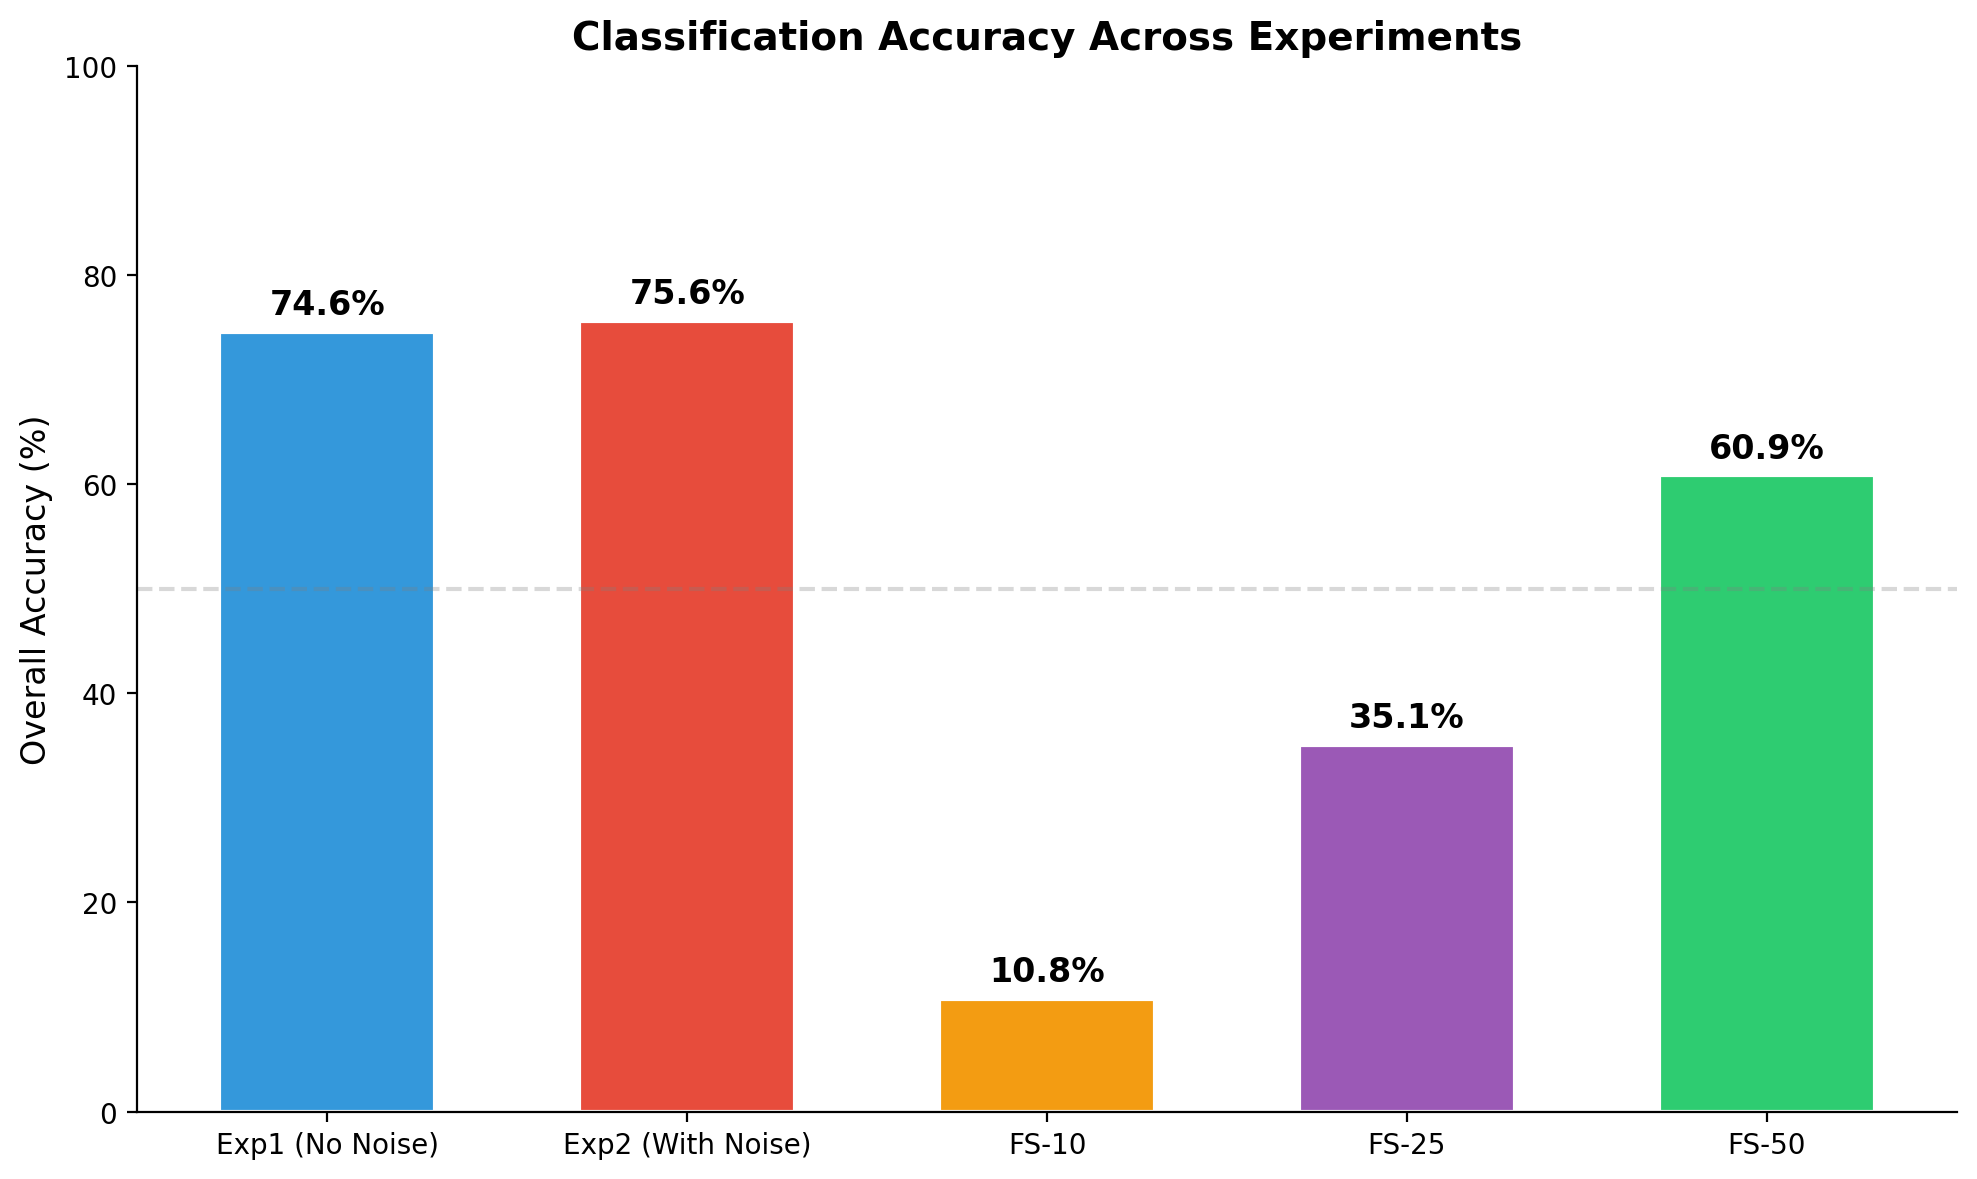
\includegraphics[width=\columnwidth]{figures/chart1_accuracy_comparison.png}}
\caption{Classification accuracy across all experimental conditions. Noise-aware fine-tuning (Exp~2) achieves the highest accuracy at 75.6\%.}
\label{fig:accuracy_comparison}
\end{figure}

The noise-aware model (Exp~2) produces 510 fewer total detections than Exp~1 (13,979 vs.\ 14,489), including 170 fewer species detections and 340 fewer mystery detections (a 10.1\% reduction). This confirms that the noise training successfully teaches the model to suppress detections on non-bird audio segments.

\subsection{Confidence Calibration}

The most striking improvement from noise-aware training is in prediction confidence. As shown in Table~\ref{tab:overall}, the median confidence increases from 0.43 (Exp~1) to 0.74 (Exp~2), representing a 71\% improvement. The proportion of high-confidence detections ($\geq$0.5) rises from 47.4\% to 60.6\%. Fig.~\ref{fig:confidence_dist} and Fig.~\ref{fig:confidence_box} illustrate the confidence score distributions and calibration across experiments.

\begin{figure}[htbp]
\centerline{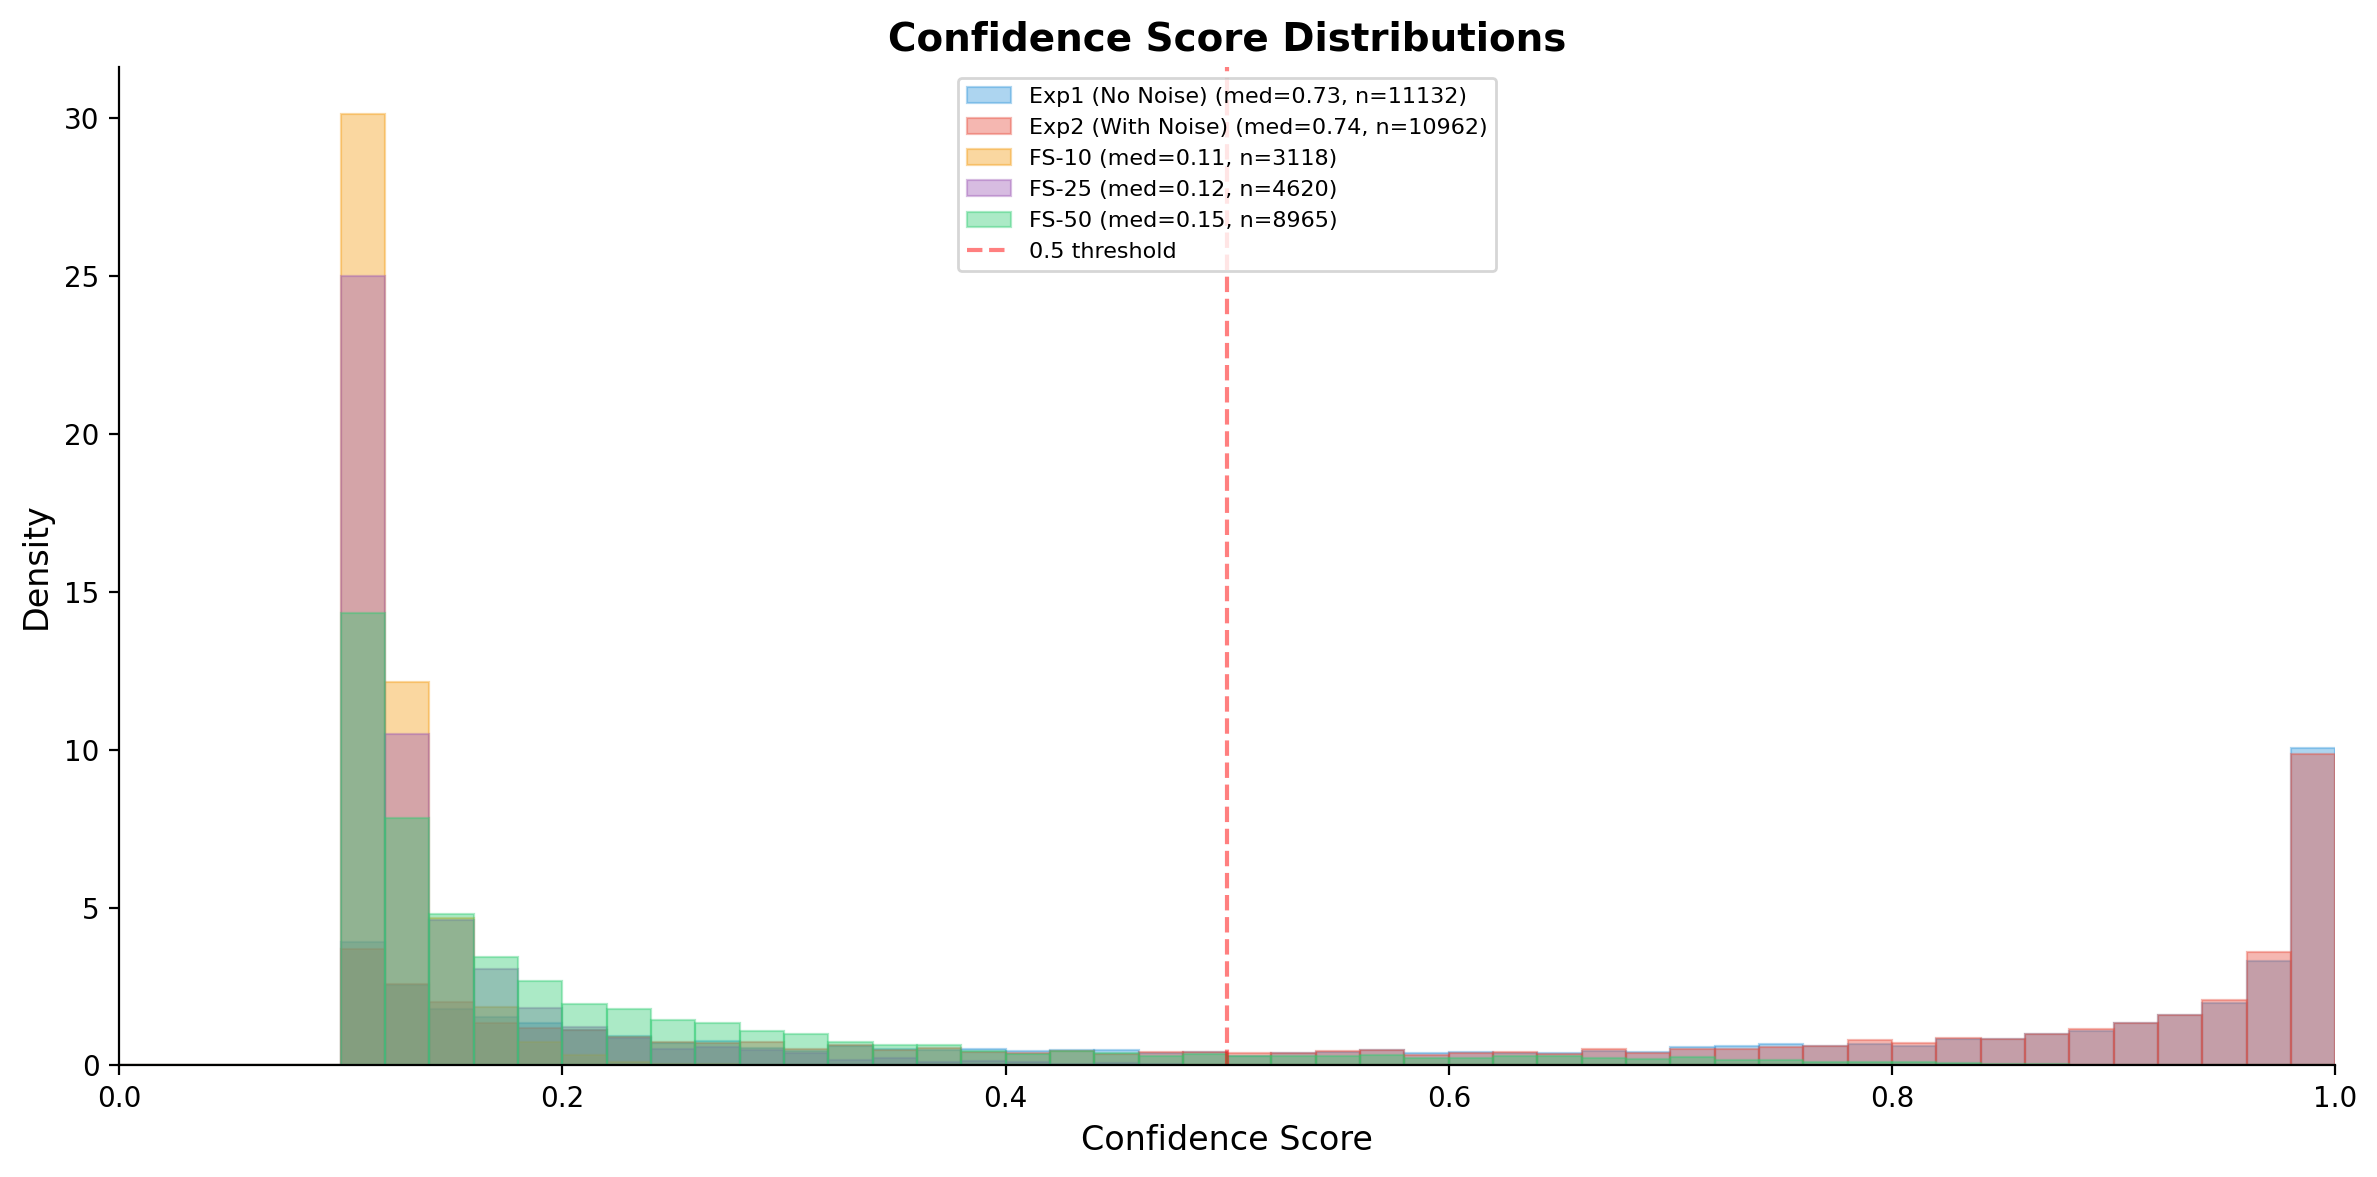
\includegraphics[width=\columnwidth]{figures/chart3_confidence_distributions.png}}
\caption{Confidence score distributions across experiments. Exp~1 and Exp~2 show high-confidence peaks near 1.0, while few-shot models cluster at low confidence values.}
\label{fig:confidence_dist}
\end{figure}

\begin{figure}[htbp]
\centerline{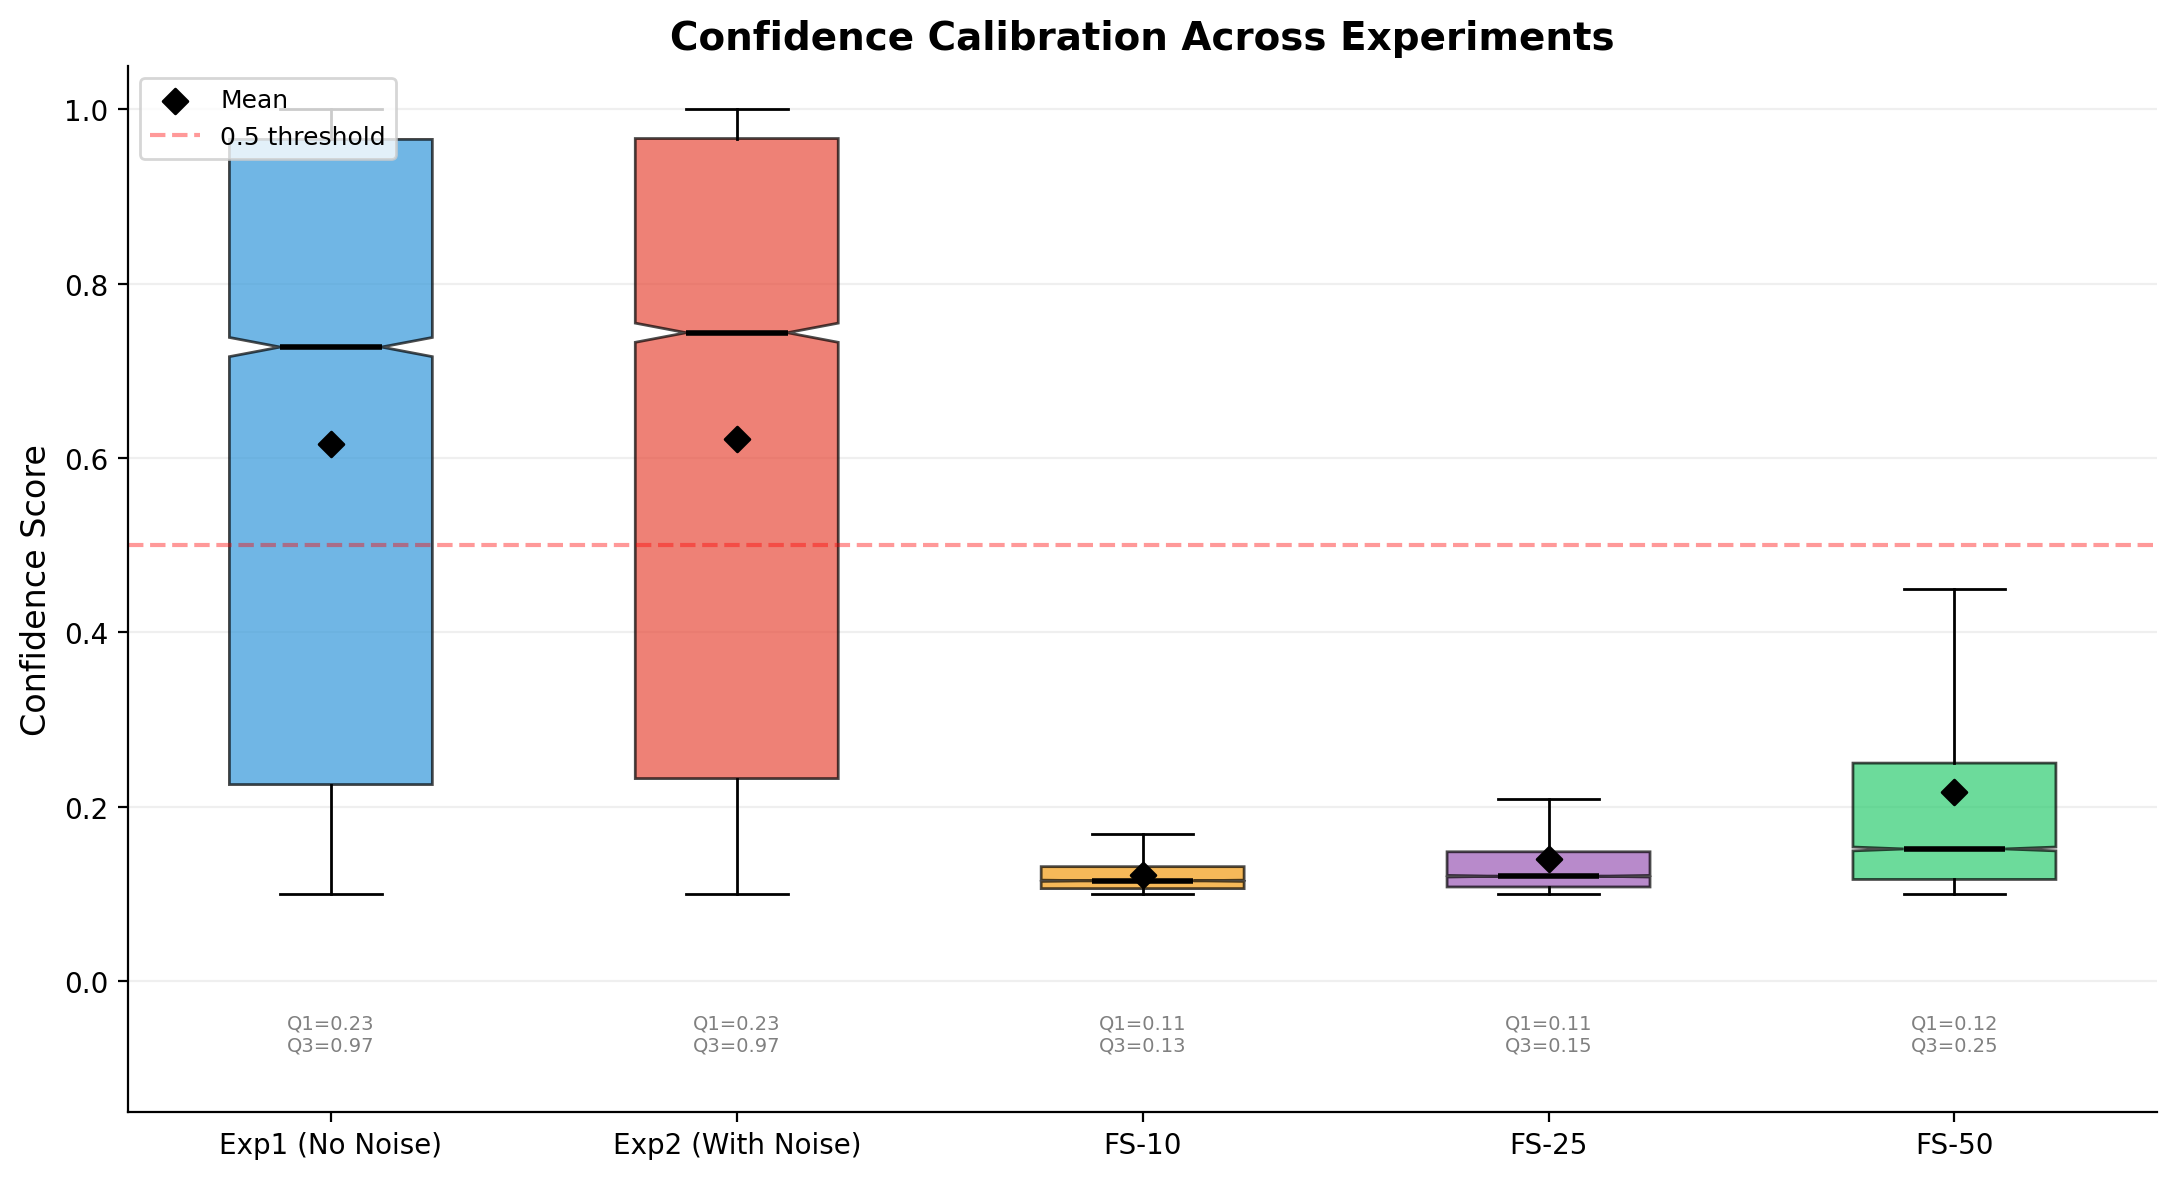
\includegraphics[width=\columnwidth]{figures/chart7_confidence_boxplots.png}}
\caption{Confidence calibration across experiments shown as box plots. Exp~2 demonstrates the highest median confidence (0.74) with the interquartile range well above the 0.5 threshold.}
\label{fig:confidence_box}
\end{figure}

In contrast, few-shot models exhibit severely degraded confidence: median values of 0.11 (FS-10), 0.12 (FS-25), and 0.15 (FS-50). Even at 50 samples per species, only 7.9\% of detections exceed 0.5 confidence, compared to 60.6\% in Exp~2.

\subsection{Impact of Noise-Aware Training on Per-Species Accuracy}

Fig.~\ref{fig:exp1_vs_exp2} presents the per-species accuracy change between Exp~1 and Exp~2. Of the 30 species, 20 showed improvement with noise-aware training, while 10 experienced slight declines.

\begin{figure}[htbp]
\centerline{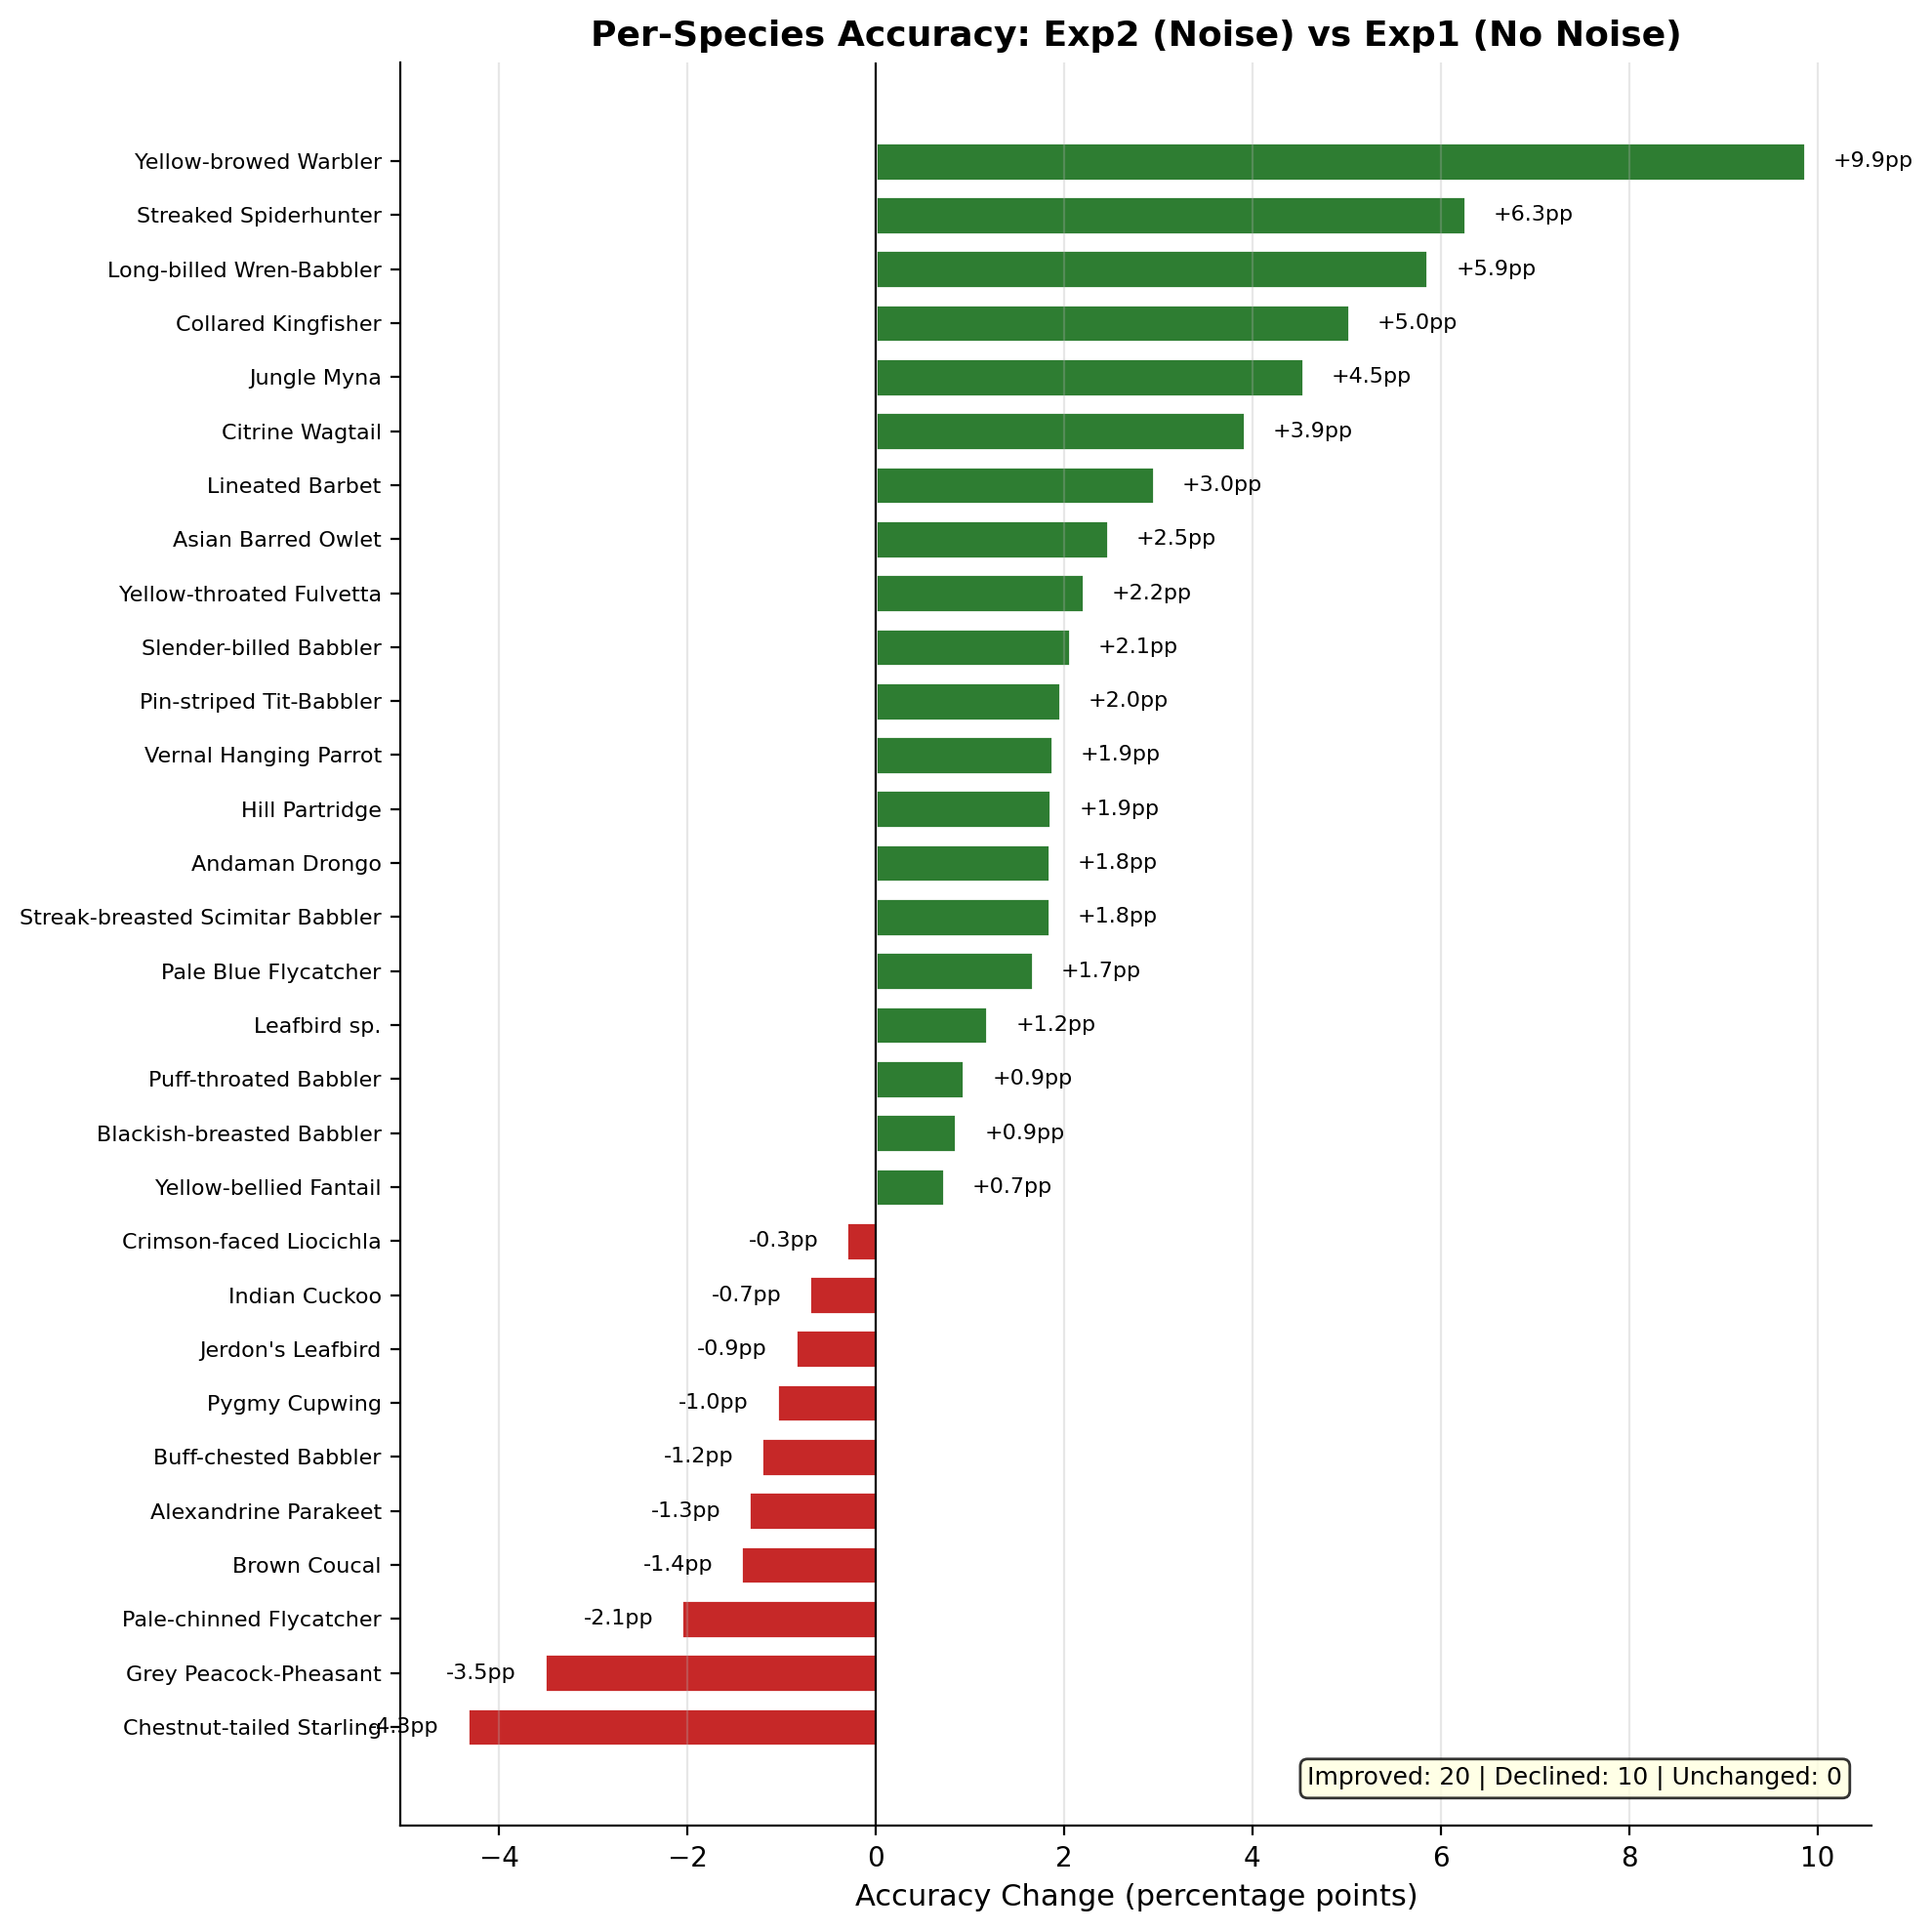
\includegraphics[width=\columnwidth]{figures/chart6_exp1_vs_exp2_delta.png}}
\caption{Per-species accuracy change from Exp~1 (no noise) to Exp~2 (with noise). Green bars indicate improvement; red bars indicate decline. 20 of 30 species improved.}
\label{fig:exp1_vs_exp2}
\end{figure}

The largest improvements were observed for Yellow-browed Warbler (+9.9pp), Streaked Spiderhunter (+6.3pp), and Long-billed Wren-Babbler (+5.9pp). The largest declines occurred for Chestnut-tailed Starling ($-$4.3pp) and Grey Peacock-Pheasant ($-$3.5pp), suggesting that these species may have borderline vocalisations that the noise filter now suppresses. Table~\ref{tab:top_species} presents the top and bottom performing species under Exp~2.

\begin{table}[htbp]
\caption{Top 5 and Bottom 5 Species by Accuracy in Exp~2}
\label{tab:top_species}
\centering
\begin{tabular}{lcc}
\toprule
\textbf{Species} & \textbf{Accuracy (\%)} & \textbf{vs Exp~1} \\
\midrule
\multicolumn{3}{l}{\textit{Top 5}} \\
Pygmy Cupwing & 90.44 & $-$1.0pp \\
Hill Partridge & 88.93 & +1.9pp \\
Asian Barred Owlet & 88.69 & +2.5pp \\
Puff-throated Babbler & 88.63 & +0.9pp \\
Citrine Wagtail & 88.46 & +3.9pp \\
\midrule
\multicolumn{3}{l}{\textit{Bottom 5}} \\
Jungle Myna & 58.71 & +4.5pp \\
Chestnut-tailed Starling & 55.43 & $-$4.3pp \\
Blackish-breasted Babbler & 52.47 & +0.9pp \\
Buff-chested Babbler & 40.39 & $-$1.2pp \\
\bottomrule
\end{tabular}
\end{table}

\subsection{Per-Species Accuracy Across All Experiments}

Fig.~\ref{fig:heatmap} presents a heatmap of per-species accuracy across all five experimental conditions, revealing species-specific sensitivity to training data volume.

\begin{figure}[htbp]
\centerline{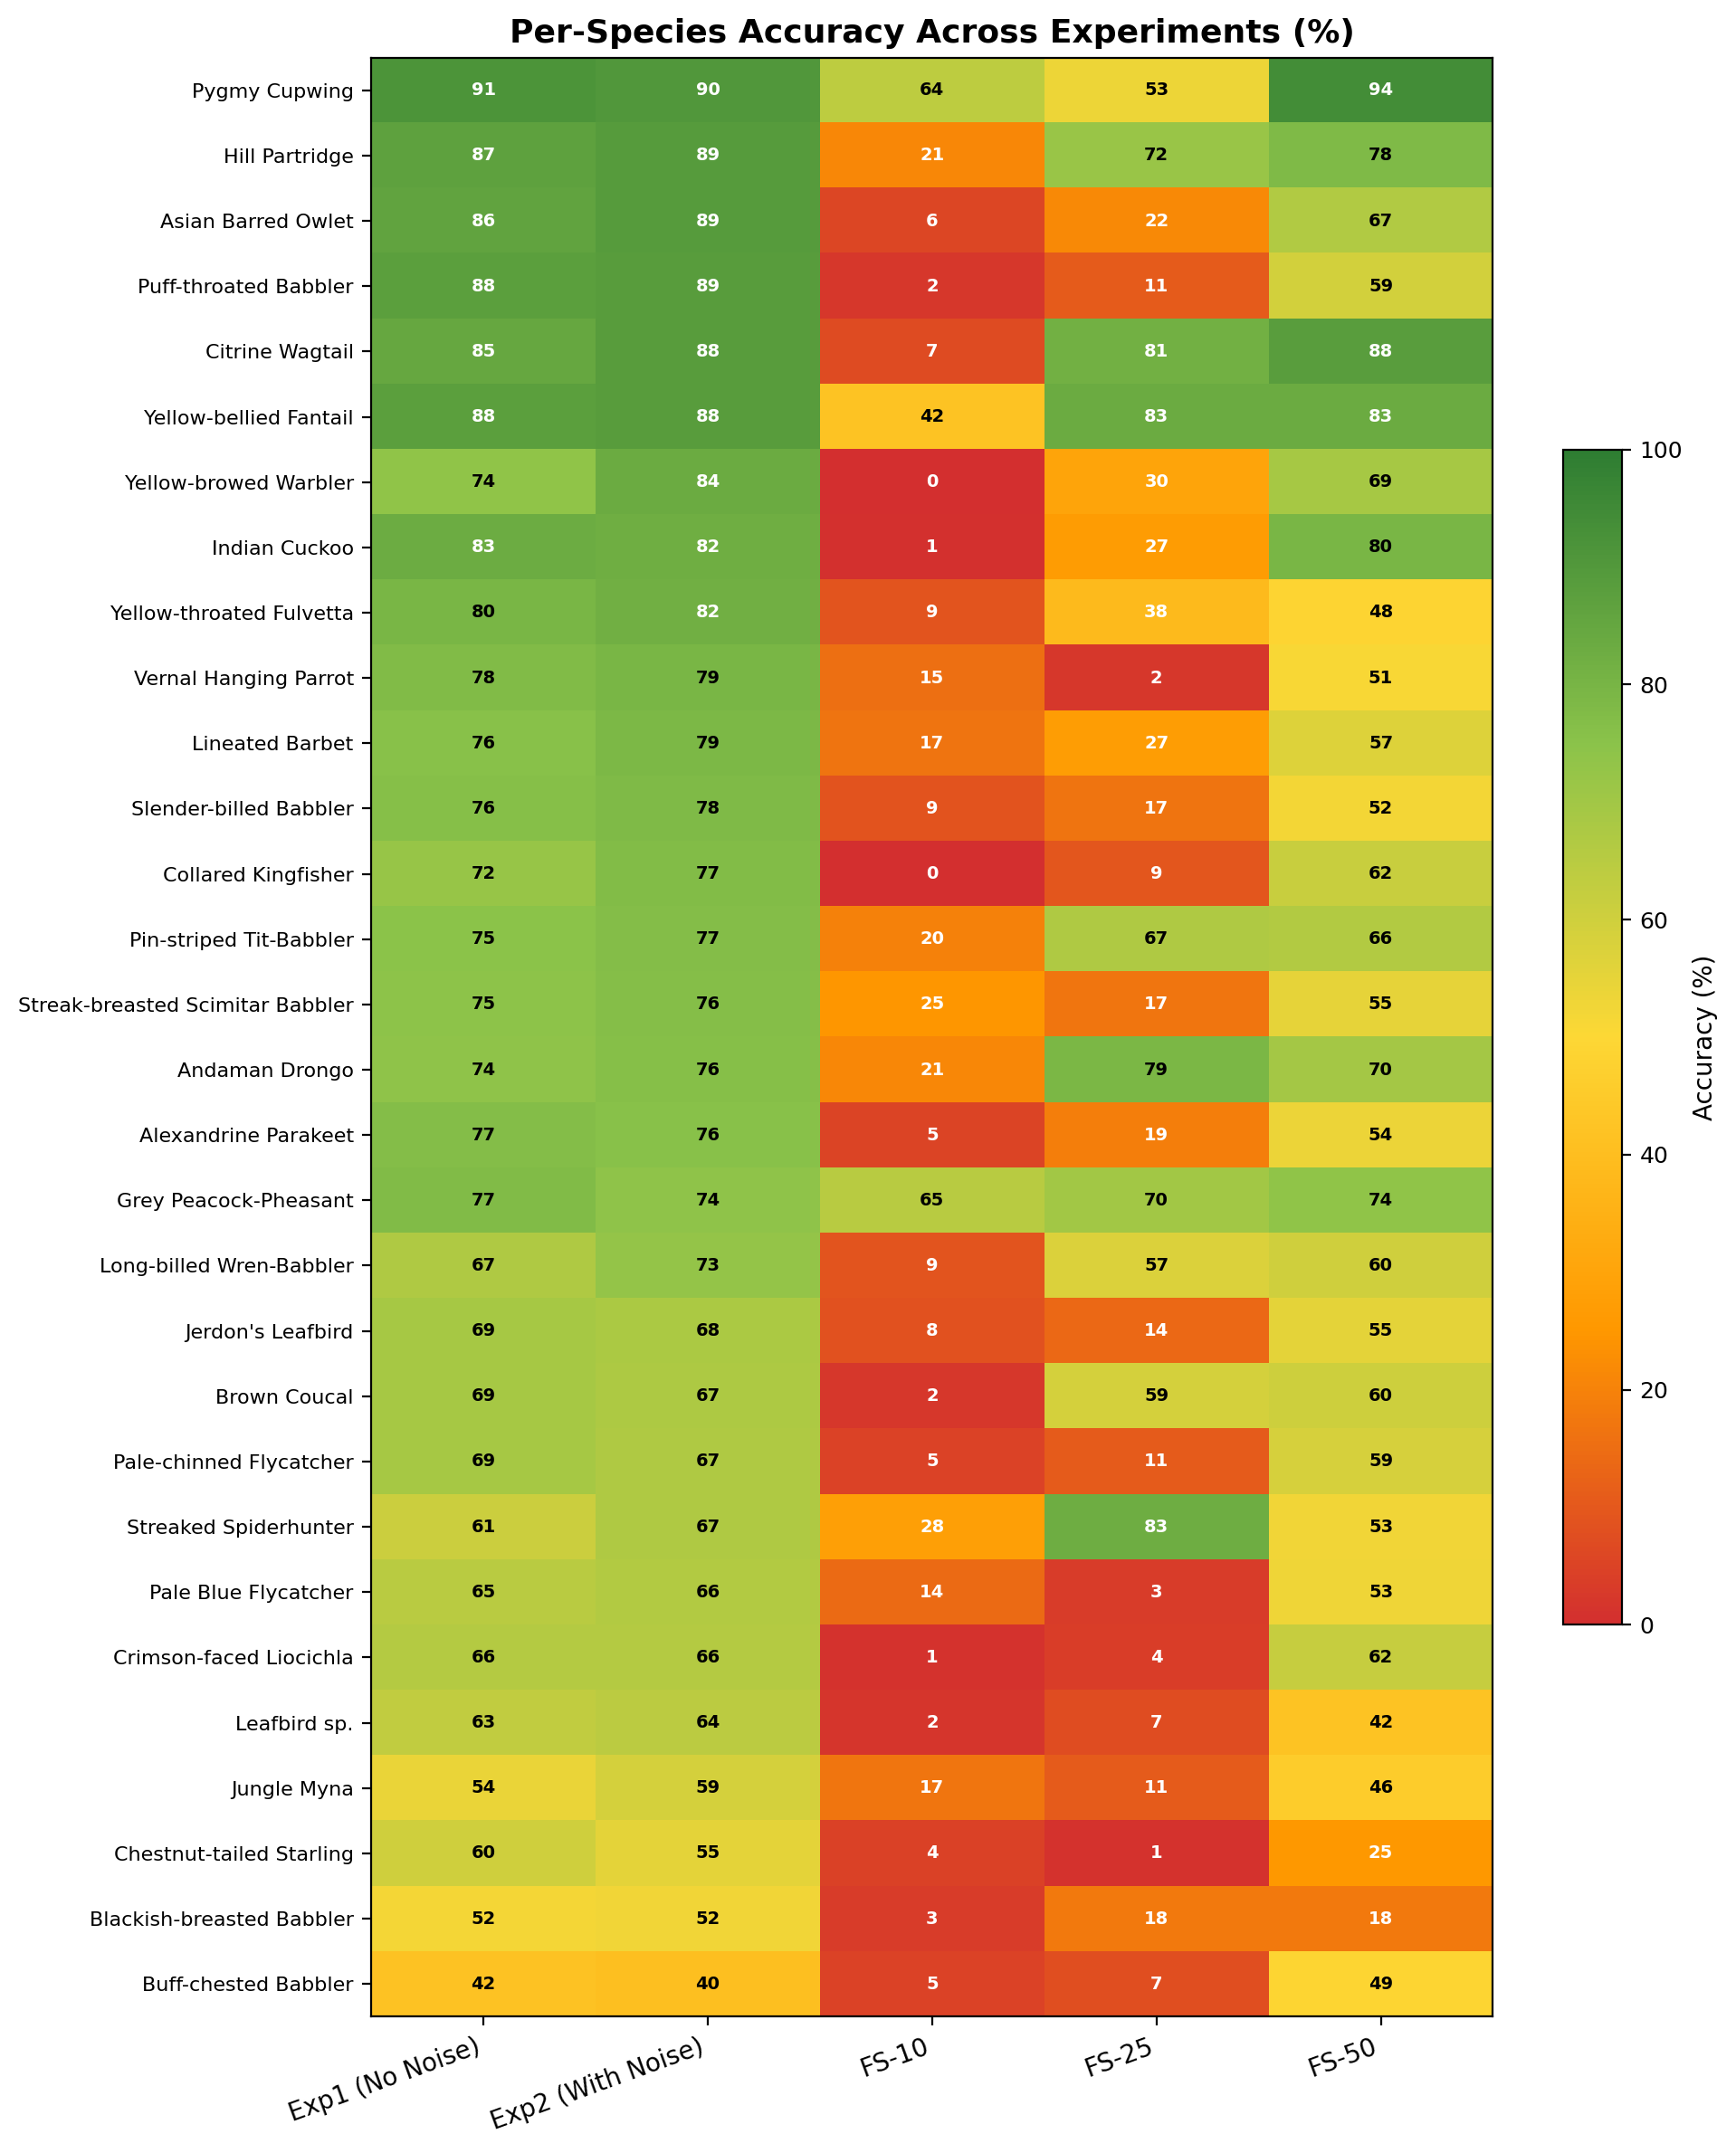
\includegraphics[width=\columnwidth]{figures/chart4_species_accuracy_heatmap.png}}
\caption{Per-species accuracy heatmap across all experiments. Species are sorted by Exp~2 accuracy (descending). Darker green indicates higher accuracy; red indicates poor performance.}
\label{fig:heatmap}
\end{figure}

Several species demonstrate robustness even under data-limited conditions. Pygmy Cupwing achieves 93.9\% accuracy at FS-50, surpassing both Exp~1 (91.5\%) and Exp~2 (90.4\%), likely due to its highly distinctive call. Conversely, data-hungry species such as Puff-throated Babbler drop from 88.6\% (Exp~2) to just 2.3\% (FS-10), indicating that species with subtle or variable vocalisations require substantially more training examples.

\subsection{Few-Shot Data Scaling}

Fig.~\ref{fig:scaling} shows the data scaling curve relating training samples per species to overall accuracy.

\begin{figure}[htbp]
\centerline{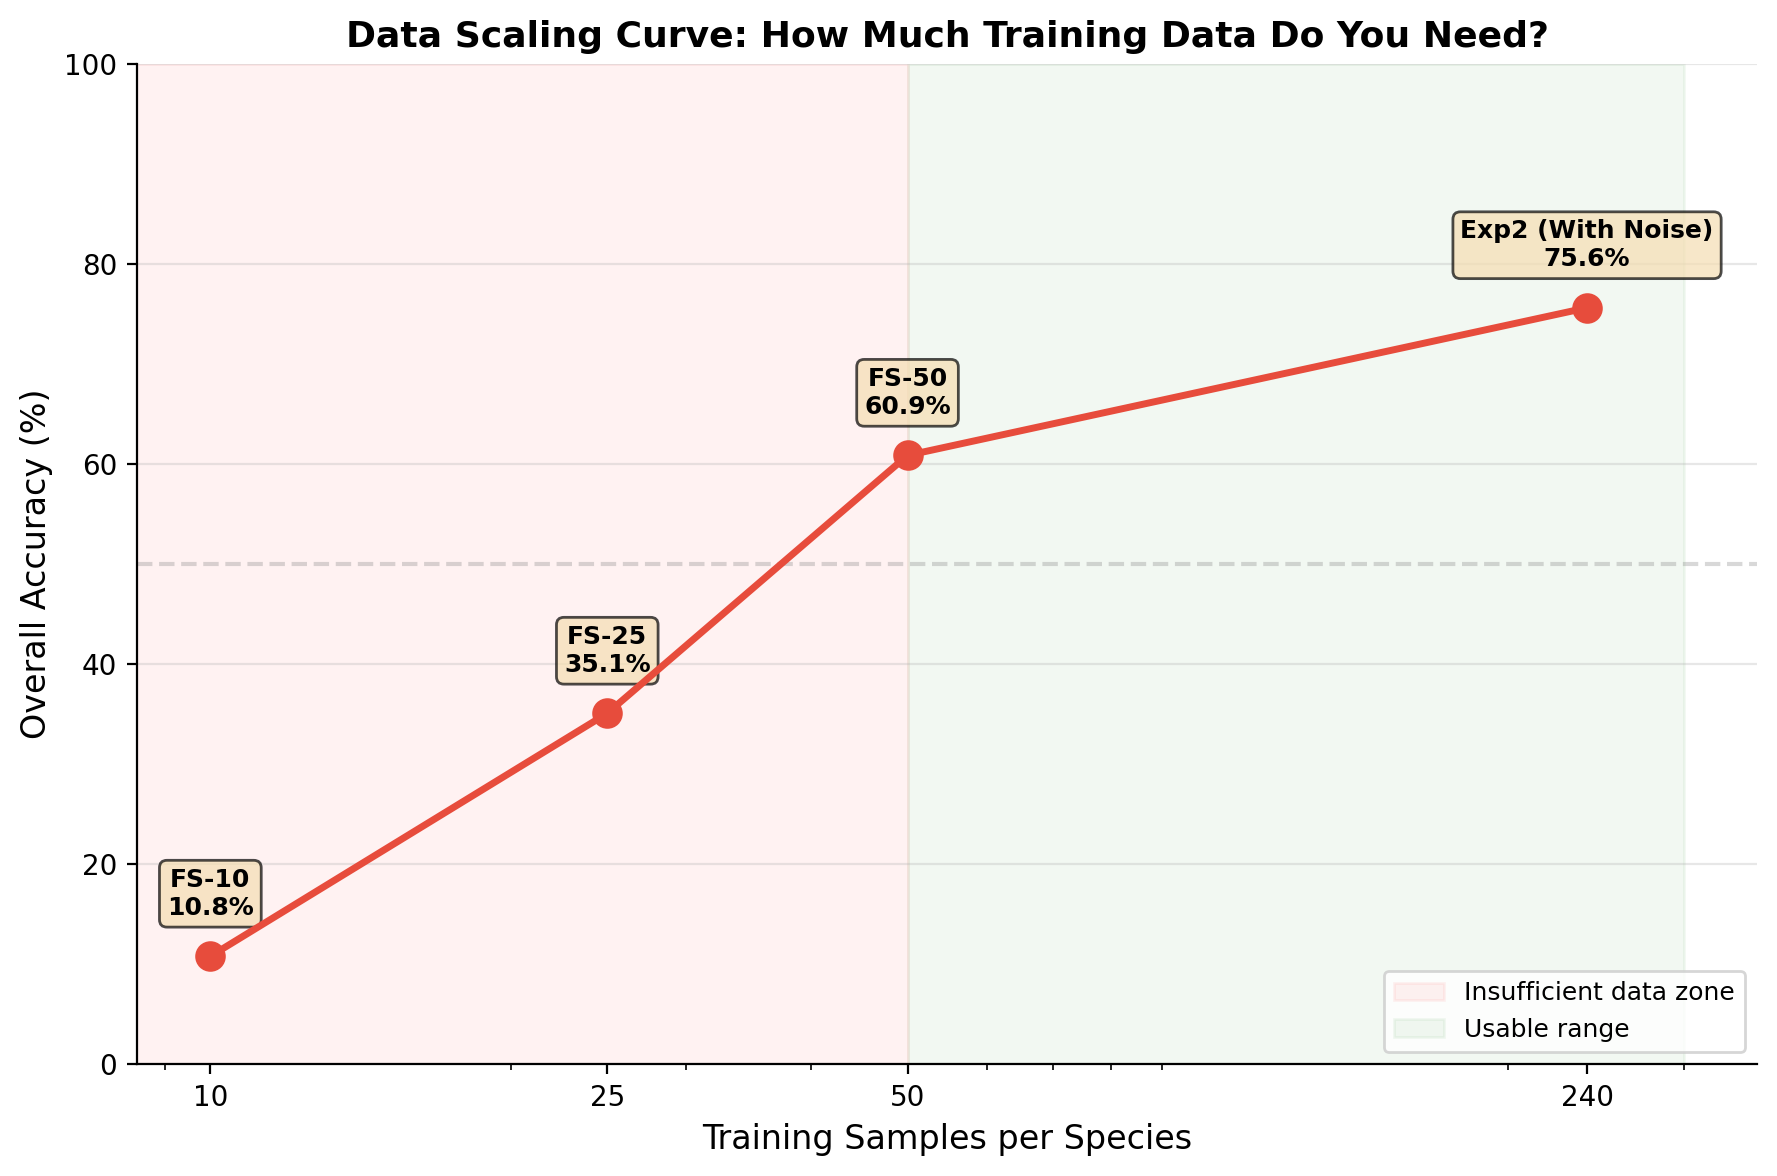
\includegraphics[width=\columnwidth]{figures/chart2_scaling_curve.png}}
\caption{Data scaling curve showing overall accuracy as a function of training samples per species. Accuracy roughly doubles with each step: 10.8\% $\rightarrow$ 35.1\% $\rightarrow$ 60.9\% $\rightarrow$ 75.6\%.}
\label{fig:scaling}
\end{figure}

The scaling relationship reveals several key findings. With 10 samples per species, accuracy is 10.81\%, essentially random performance, confirming that BirdNET cannot learn meaningful species features from just 10 examples. At 25 samples, accuracy reaches 35.09\% with extreme variance across species --- distinctive callers such as Chelidorhynx hypoxanthus (83.4\%) and Motacilla citreola (81.4\%) perform well while many species fail. At 50 samples, accuracy reaches 60.86\%, a meaningful classifier but still 14.75pp below the full dataset. The curve suggests diminishing returns above approximately 100 samples per species but severe degradation below 50.

\subsection{Confusion Analysis}

Fig.~\ref{fig:confusion} presents the row-normalised confusion matrix for Exp~2. The dominant misclassification patterns involve acoustically similar species, particularly within the babbler family (Timaliidae).

\begin{figure}[htbp]
\centerline{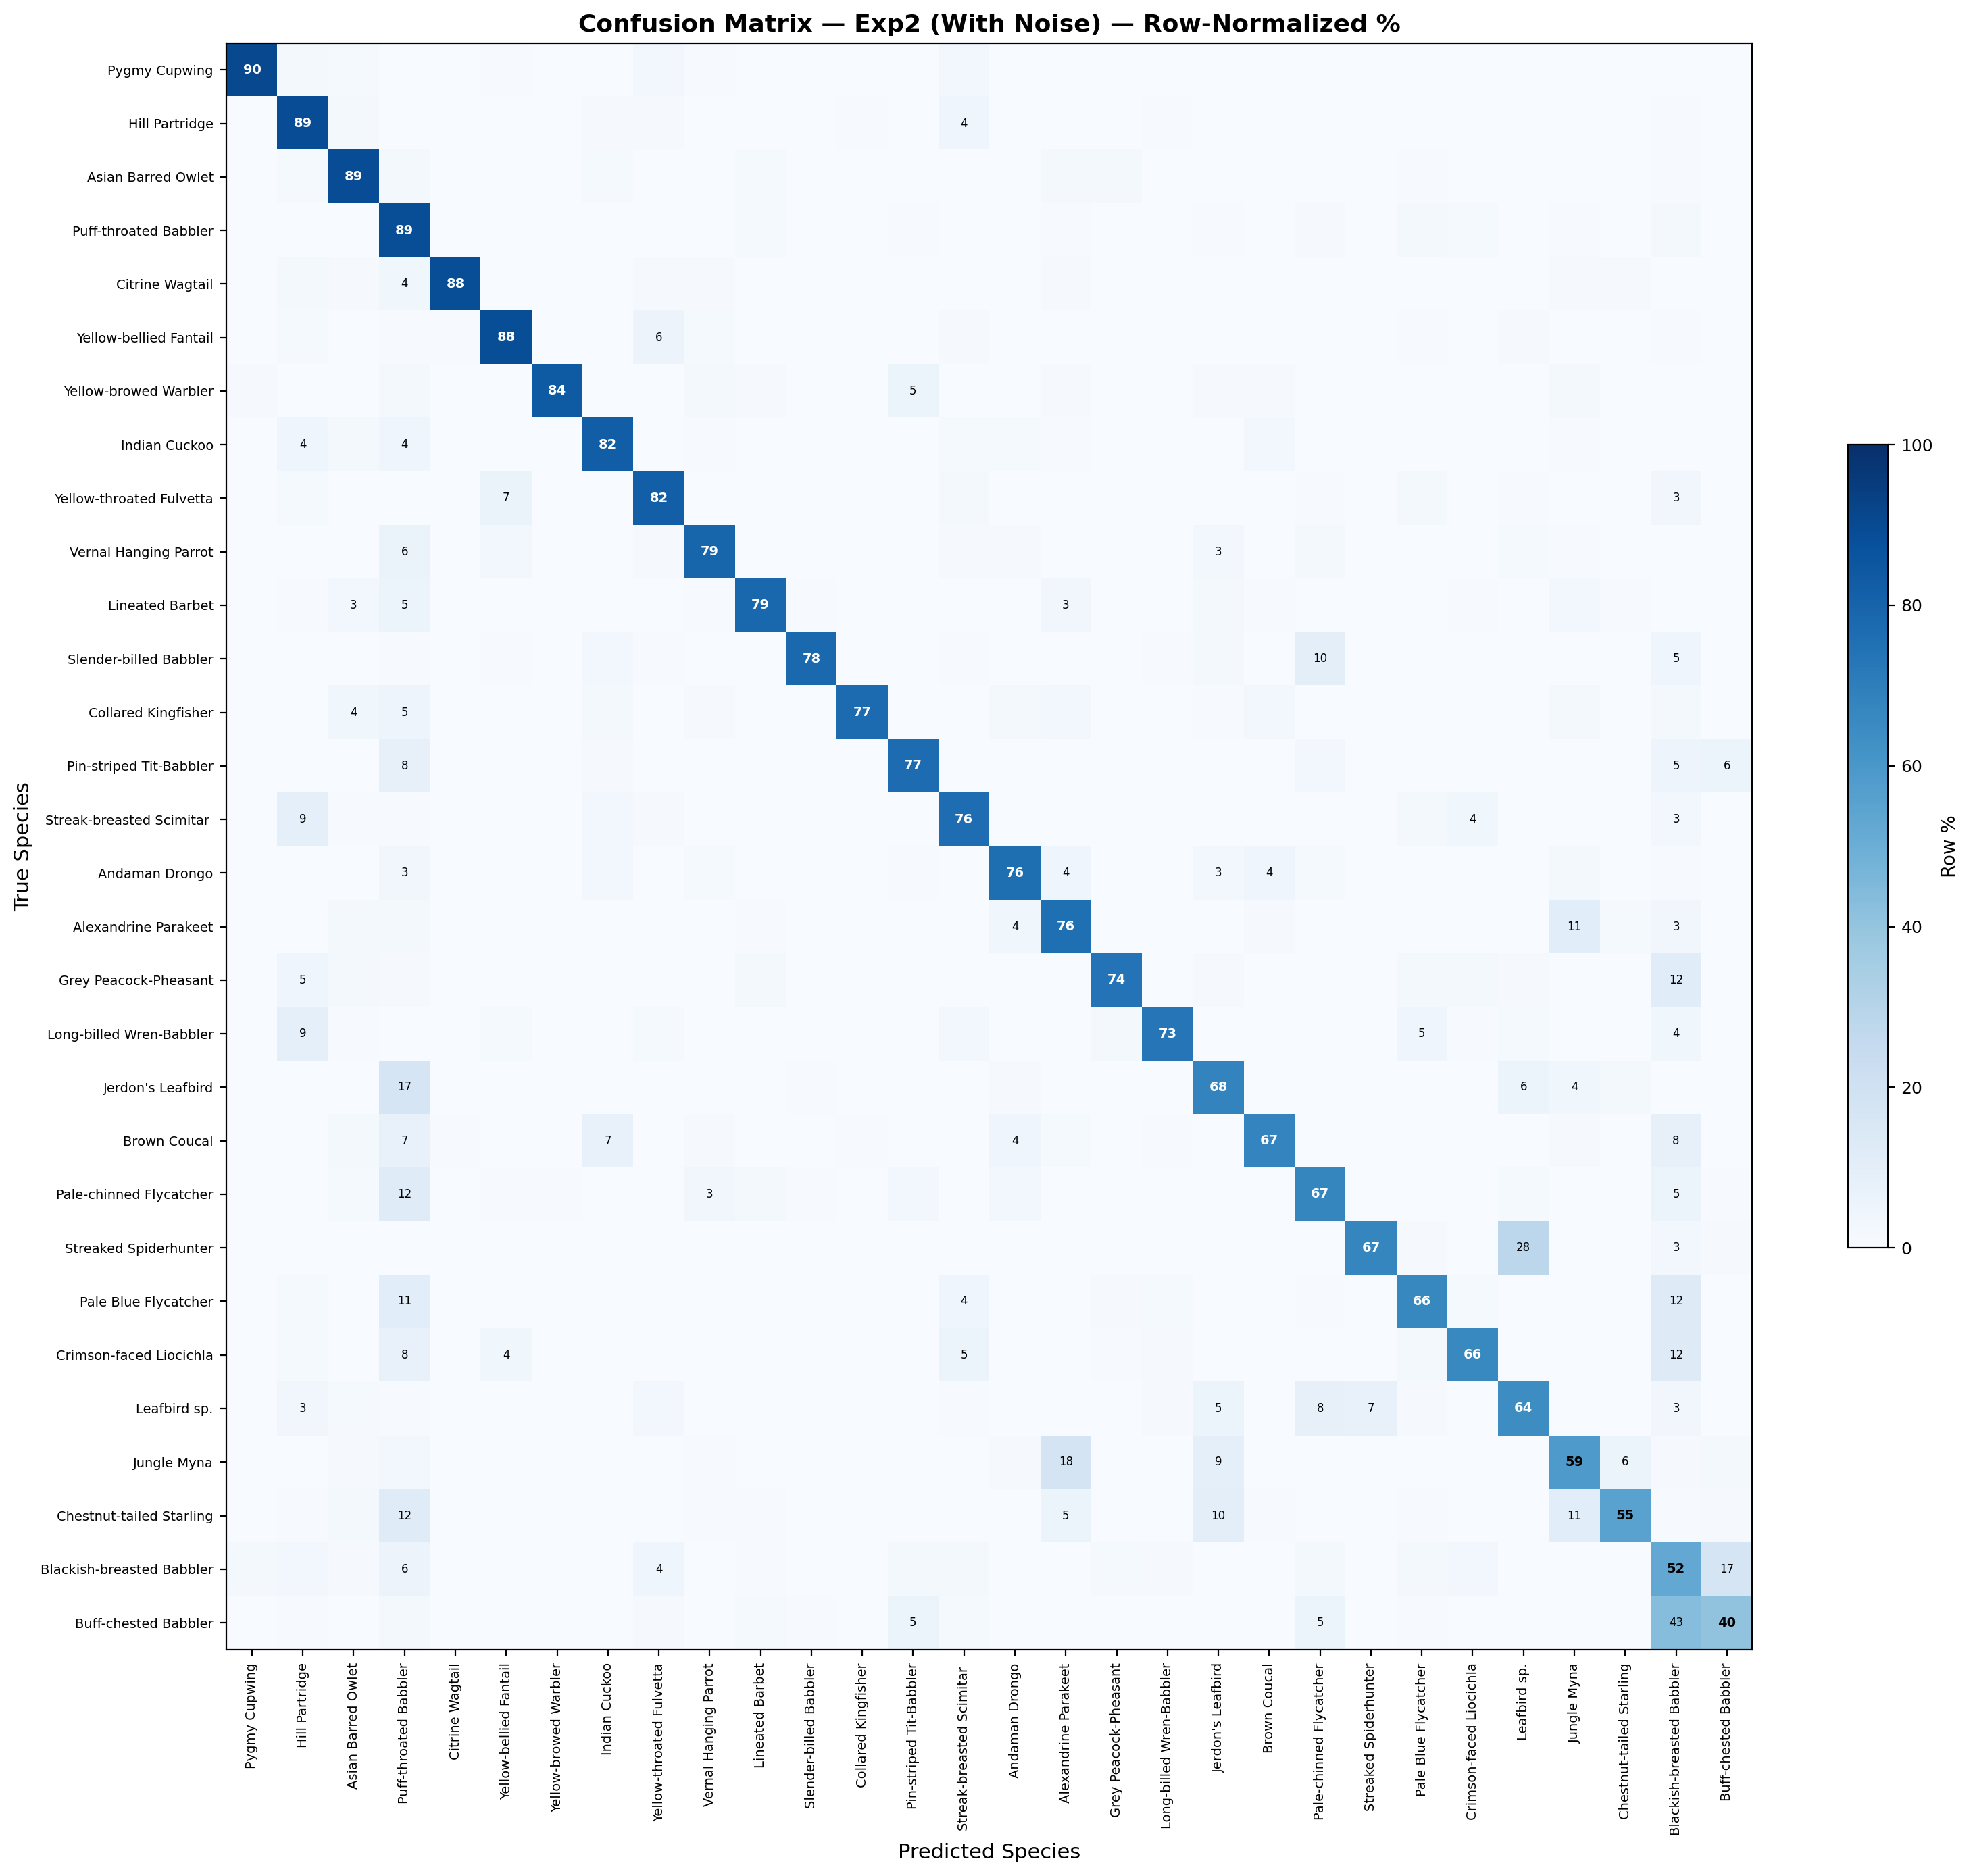
\includegraphics[width=\columnwidth]{figures/chart5_confusion_matrix_exp2.png}}
\caption{Row-normalised confusion matrix for Exp~2 (with noise). Strong diagonal indicates good overall classification; off-diagonal clusters reveal systematic inter-species confusion, particularly among babblers.}
\label{fig:confusion}
\end{figure}

Table~\ref{tab:confusion} lists the top misclassification pairs. The Stachyridopsis ambigua--Sphenocichla humei pair dominates with 110 and 102 bidirectional misclassifications, indicating high spectral overlap between these babbler species.

\begin{table}[htbp]
\caption{Top 10 Misclassification Pairs in Exp~2}
\label{tab:confusion}
\centering
\begin{tabular}{llc}
\toprule
\textbf{True Species} & \textbf{Predicted As} & \textbf{Count} \\
\midrule
Stachyridopsis ambigua & Sphenocichla humei & 110 \\
Sphenocichla humei & Stachyridopsis ambigua & 102 \\
Cyornis unicolor & Sphenocichla humei & 75 \\
Cyornis unicolor & Pellorneum ruficeps & 66 \\
Pomatorhinus ruficollis & Arborophila torqueola & 58 \\
Liocichla phoenicea & Sphenocichla humei & 55 \\
Cyornis poliogenys & Pellorneum ruficeps & 50 \\
Chloropsis jerdoni & Pellorneum ruficeps & 45 \\
Acridotheres fuscus & Psittacula eupatria & 36 \\
Liocichla phoenicea & Pellorneum ruficeps & 35 \\
\bottomrule
\end{tabular}
\end{table}

The persistence of babbler confusion across both Exp~1 and Exp~2 --- despite the addition of noise training --- confirms that this is a species-similarity problem rooted in spectral overlap rather than a noise-related artefact. This represents a fundamental limitation that cannot be resolved through data engineering alone and would require architectural modifications such as attention-based temporal modelling.

\subsection{Training Convergence}

Experiment~2 achieved a best AUPRC of 0.961, AUROC of 0.997, and a best loss of 0.715 at epoch 50/50, indicating strong convergence and effective model selection through the AUPRC criterion.

% ============================================================
% VI. DISCUSSION
% ============================================================
\section{Discussion}

\subsection{Effectiveness of Noise-Aware Training}

As can be observed, the inclusion of environmental noise samples from ESC-50 leads to clear performance gains in both accuracy (+1.05pp) and confidence calibration (+71\% median confidence). Here, the noise class serves as the \texttt{NON\_EVENT\_CLASS} in the training process, making the model learn to use the learned internal representation to inhibit any detection on the non-bird audio parts. This fact is corroborated by the 10.1\% decline in the number of detections in the mystery folder (from 3,357 to 3,017).

Even though the improvement in the absolute accuracy value is modest, there is a significant change in the way the confidence distribution looks like. Specifically, the increase in median confidence from 0.43 to 0.74 implies that the model becomes more confident in its predictions, making sure that it is not wrong about them most of the time. In practice, that means that when setting the detection threshold to 0.5, the proportion of detections retained is 60.6\% in Experiment~2 versus 47.4\% in Experiment~1.

\subsection{Data Efficiency and Few-Shot Drawbacks}

From the few-shot studies, there is a dramatic trend of data efficiency, such that the model's performance doubles (from 10.8\% to 35.1\%, then 60.9\%, and finally 75.6\%) at each stage. The most crucial insight here is that ten samples per species are insufficient and yield a random prediction. With fifty samples per species, the model performs 60.86\% accurately, which can be considered functional classification, albeit with greatly reduced confidence (median: 0.15 vs.\ 0.74 from full datasets).

At the species level, we observe that certain species with unique vocal signatures (for instance, Pygmy Cupwing and Grey Peacock-Pheasant) can withstand low data, whereas other species with ambiguous callings (for example, Puff-throated Babbler and \textit{Pellorneum ruficeps}) need much higher samples. It is evident that an adaptive sampling scheme based on individual species characteristics is beneficial in the data gathering process.

\subsection{Confusion Patterns Between Species}

Since the confusion between different babbler species (\textit{Stachyridopsis ambigua}, \textit{Sphenocichla humei}, and \textit{Pellorneum ruficeps}) persists under all tested conditions, it is safe to conclude that this phenomenon is an intrinsic issue stemming from spectral similarity between species in the Timaliidae family. The frequency bands and temporal patterns used by these species overlap, thus making the task of differentiating the species based on spectrograms alone impossible.

In essence, the above conclusion marks the demarcation line between improving data engineering and enhancing the network architecture itself. Although noise-aware training solves the issue of poor performance due to noise, the resolution of babbler confusion will likely require changes to the architecture of the network.

\subsection{Limitations}

Several limitations should be acknowledged. First, the IBC53 dataset contains only 30 of India's 1,350+ bird species, limiting the generalisability of the findings. Second, the ESC-50 noise categories, while relevant, may not fully represent the diversity of environmental noise encountered in Indian field recordings. Third, the evaluation uses BirdNET's built-in inference pipeline, which processes 3-second windows independently without temporal context across adjacent segments. Finally, the few-shot experiments use random sampling without stratification by recording quality or vocalisation type, which may introduce sampling bias.

% ============================================================
% VII. CONCLUSION
% ============================================================
\section{Conclusion}

This paper presented a noise-aware fine-tuning framework for adapting BirdNET to classify 30 Indian bird species using the IBC53 dataset. The proposed four-stage CST pipeline --- comprising audio segmentation, energy-based noise detection, noise-augmented dataset construction, and BirdNET fine-tuning --- demonstrates that incorporating environmental noise from ESC-50 into the training process improves classification accuracy from 74.56\% to 75.61\% while increasing median prediction confidence by 71\% (from 0.43 to 0.74) and reducing false detections by 510.

Few-shot experiments establish that 50 labelled samples per species provide 60.86\% accuracy, identifying a practical minimum dataset size threshold for BirdNET fine-tuning. The analysis further reveals that persistent confusion between morphologically similar babbler species (Timaliidae) represents a spectral similarity limitation that cannot be addressed through data engineering alone.

Future work should explore attention-based temporal modelling to resolve inter-species confusion, species-adaptive confidence thresholds for deployment optimisation, expanded noise augmentation with region-specific environmental recordings, and scaling the framework to the full IBC53 dataset of 53 species.

% ============================================================
% REFERENCES
% ============================================================
\begin{thebibliography}{00}
\bibitem{b1} S. Kahl, C. M. Wood, M. Eibl, and H. Klinck, ``BirdNET: A deep learning solution for avian diversity monitoring,'' \textit{Ecological Informatics}, vol.~61, p.~101236, 2021.
\bibitem{b2} K. J. Piczak, ``ESC: Dataset for environmental sound classification,'' in \textit{Proc. 23rd ACM Int. Conf. Multimedia}, 2015, pp.~1015--1018.
\bibitem{b3} A. Sahoo, ``IBC53: Indian Bird Call Dataset,'' Kaggle, 2024. [Online]. Available: \url{https://www.kaggle.com/datasets/arghyasahoo/ibc53-indian-bird-call-dataset}
\bibitem{b4} T. M. Aide, C. Corrada-Bravo, M. Campos-Cerqueira, C. Milan, G. Vega, and R. Alvarez, ``Real-time bioacoustics monitoring and automated species identification,'' \textit{PeerJ}, vol.~1, p.~e103, 2013.
\bibitem{b5} J. Sueur and A. Farina, ``Ecoacoustics: the ecological investigation and interpretation of environmental sound,'' \textit{Biosemiotics}, vol.~8, no.~3, pp.~493--502, 2015.
\bibitem{b6} V. Lostanlen, J. Salamon, A. Farnsworth, S. Kelling, and J. P. Bello, ``Birdvox-Full-Night: A dataset and benchmark for avian flight call detection,'' in \textit{Proc. IEEE ICASSP}, 2019, pp.~266--270.
\bibitem{b7} C. Rasmussen and J. C. Anderton, \textit{Birds of South Asia: The Ripley Guide}, 2nd~ed. Washington, DC: Smithsonian Institution, 2012.
\bibitem{b8} S. J. Pan and Q. Yang, ``A survey on transfer learning,'' \textit{IEEE Trans. Knowl. Data Eng.}, vol.~22, no.~10, pp.~1345--1359, Oct. 2010.
\bibitem{b9} Fairbrass, A. J. \textit{et al.}, ``BirdNET accuracy assessment,'' 2025.
\bibitem{b10} Petry, L. \textit{et al.}, ``Species-specific confidence thresholds for BirdNET,'' 2026.
\bibitem{b11} Winiarska, D. \textit{et al.}, ``Comparison of point counts, PAM, and BirdNET in Bia\l{}owie\.{z}a forest,'' 2025.
\bibitem{b12} P\'{e}rez-Granados, C. \textit{et al.}, ``World-wide BirdNET assessment,'' 2025.
\bibitem{b13} Tseng, Y. \textit{et al.}, ``Species-specific thresholds for BirdNET in western Canada,'' 2025.
\bibitem{b14} Iglesias-Merchan, C. \textit{et al.}, ``PAM and BirdNET for wetland bird inventory,'' 2026.
\bibitem{b15} Allen-Ankins, S. \textit{et al.}, ``BirdNET embeddings for novel sound class identification,'' 2025.
\bibitem{b16} Assarzadeh, S. \textit{et al.}, ``Explaining BirdNET misclassifications using XAI,'' 2025.
\bibitem{b17} P\'{e}rez-Granados, C. \textit{et al.}, ``Assessing BirdNET for Neotropical wetland birds,'' 2025.
\bibitem{b18} Mei, Z. \textit{et al.}, ``BirdNET and Random Forest for Chinese Bamboo Partridge detection,'' 2026.
\bibitem{b19} Seye, M. \textit{et al.}, ``IoT-based gull monitoring with BirdNET,'' 2025.
\bibitem{b20} Schiavo, G. \textit{et al.}, ``Fine-tuning BirdNET for Alpine bird species,'' 2025.
\bibitem{b21} Fradet, L. \textit{et al.}, ``Custom BirdNET classifier for wind noise in Ad\'{e}lie penguin recordings,'' 2025.
\end{thebibliography}

\end{document}
